\documentclass[12pt, a4paper,oneside, nocenter]{thesis}

%setting font to Arial and using UTF-8
\usepackage[utf8]{inputenc}
\usepackage[T1]{fontenc}
\usepackage[scaled]{uarial}
\renewcommand*\familydefault{\sfdefault} 

\usepackage{amsfonts}%checkmark

\usepackage{graphicx}%package for imges 
\usepackage{float}

\usepackage{tabularx}%table package
\usepackage{lastpage}%get page count
\usepackage{makecell}%multiline cell
\usepackage{multirow}%multirow
\usepackage{pdflscape}%for one page table

%centered columns P%
\usepackage{array}
%horizontal
\newcolumntype{P}[1]{>{\centering\arraybackslash}p{#1}}
%vertical
\newcolumntype{M}[1]{>{\centering\arraybackslash}m{#1}}

\usepackage{soul}
\usepackage[hyphens]{url}
\def\UrlBreaks{\do\/\do-}
\usepackage[hyphenbreaks]{breakurl}
\urlstyle{same}

\usepackage[normalem]{ulem}
\usepackage[dvipsnames]{xcolor}

\usepackage{etoolbox}
\usepackage{setspace}
\usepackage{wallpaper}
\usepackage{lipsum}
\usepackage{eurosym}
%\usepackage[none]{hyphenat}
%remove hyphenation
\tolerance=1
\emergencystretch=\maxdimen
\hyphenpenalty=10000
\hbadness=10000

\usepackage[document]{ragged2e}
\usepackage[font=small,labelfont=normal,figurename=Figure,labelsep=period]{caption} % Required for specifying captions to tables and figures
\captionsetup{justification=raggedright,singlelinecheck=false}

\usepackage[margin=1in,top=0.5in,includehead=true]{geometry}
%TOC links
\usepackage[hyperfootnotes=false]{hyperref}%
\hypersetup{
    colorlinks,
    citecolor=black,
    filecolor=black,
    linkcolor=black,
		urlcolor=blue,
		linktoc=all
}
\definecolor{green}{rgb}{1,0.5,0}

\definecolor{red}{rgb}{1,0.5,0}

\newcommand{\urlul}[1]{\url{\color{green}\setulcolor{red}\ul{#1}}}

\usepackage{cleveref}%setting figure and table referencing
\crefname{figure}{(Figure}{(Figure}
\crefname{table}{(Table}{(Table}
\creflabelformat{table}{#2\textup{#1}#3)}
\creflabelformat{figure}{#2\textup{#1}#3)}
%%%%%%%%%%%%%%%%%%%%%%

\usepackage{titlesec}
\assignpagestyle{\chapter}{fancy}

% \ignore command for inline comments
\newcommand{\ignore}[2]{\hspace{0in}#2}

%Setting new line margins
\renewcommand{\baselinestretch}{1.5}

% package for todonotes
\usepackage[colorinlistoftodos,prependcaption,textsize=tiny]{todonotes}

% some colours
\definecolor{olive}{rgb}{0.5, 0.5, 0.0}
\newcommand{\info}[2][1=]{\todo[linecolor=olive,backgroundcolor=olive!25,bordercolor=olive,#1]{#2}}
\newcommand{\improvement}[2][1=]{\todo[linecolor=Plum,backgroundcolor=Plum!25,bordercolor=Plum,#1]{#2}}

\renewcommand{\chaptername}{CHAPTER}

\usepackage{tocloft}%changing table of contents to dots

\renewcommand{\cftdotsep}{1} % smaller dot spacing
\renewcommand{\cftsecleader}{\cftdotfill{\cftdotsep}} % for sections
\renewcommand{\cftpartleader}{\cftdotfill{\cftdotsep}} % for parts
\renewcommand{\cftchapleader}{\cftdotfill{\cftdotsep}} % for chapters
\renewcommand\cftchapfont{\normalfont\fontsize{12}{12}\selectfont} % chapter font to 12\12
\renewcommand\cftchappagefont{\normalfont\fontsize{12}{12}\selectfont} %chapter page number font to 12\12

%headheight resetting error
\setlength{\headheight}{15pt}% ...at least 51.60004pt
%disabling identation for paragraphs
\setlength{\parindent}{0cm}
%increasing space before chapter
\setlength{\cftbeforechapskip}{2.5pt}

%style for chapters
\titleformat{\chapter}
[hang]
{\normalfont\fontsize{12}{12}\selectfont\bfseries}
{\thechapter}
{1em}{}

\titlespacing*{\chapter}{0pt}{-0.2cm}{0.3cm}
\titleformat*{\section}{\normalfont\fontsize{12}{12}\selectfont\bfseries}
\titleformat*{\subsection}{\normalfont\fontsize{12}{12}\selectfont\bfseries}
\titleformat*{\subsubsection}{\normalfont\fontsize{12}{12}\selectfont\bfseries}
\setlength{\parskip}{1em}

\usepackage{fancyhdr}%fancy headers/footers

\fancyhf{} % sets both header and footer to nothing
\fancyhead[C]{\thepage}

\fancypagestyle{plain}{%
\fancyhf{} % clear all header and footer fields
\fancyhead[C]{\thepage} %RO=right odd, RE=right even
\renewcommand{\headrulewidth}{0pt}
\renewcommand{\footrulewidth}{0pt}
}
%-- Stop figure counter resetting --%
\usepackage{chngcntr}
 
\counterwithout{figure}{chapter}
\counterwithout{table}{chapter}
\renewcommand{\tableshortname}{Table}

\setcounter{section}{1}%start table of contents at 1
\usepackage{xstring}
\newcommand{\cleanul}[1]{%
    \StrSubstitute{#1}{\_}{\textvisiblespace}%
}%
%-----------------------------------References------------------------------%
\usepackage[nottoc,notlot,notlof]{tocbibind}
\usepackage[]{natbib}
\usepackage{usebib}
\newbibfield{title}
\newbibfield{year}
\newbibfield{author}
\bibinput{references}

% date fixing for citations
\def\changeformat#1{\xchangeformat#1\relax}
\def\xchangeformat#1-#2-#3\relax{%
#3 %
\ifcase#2 \or
January\or February\or March\or April\or May\or June\or July\or
August\or September\or October\or November\or December\fi
\ #1}

%custom bibliography style and citation commands
\bibliographystyle{xamk}
%\bibliographystyle{plainnat}

%\renewcommand{\citep}[1]{(\citealp{#1}.)}
%\newcommand{\citeyearxamk}[1]{(\citeyear{#1}.)}
\newcommand{\citeyearxamk}[1]{(\citeauthor{#1} \citeyear{#1})}
\renewcommand{\citep}[1]{(\citeauthor{#1} \citeyear{#1}.)}
\renewcommand{\citeyearpar}[1]{(\citeauthor{#1} \citeyear{#1})}
\newcommand{\citeyeartitlexamk}[1]{(\usebibentry{#1}{title} \citeyear{#1}.)}
\newcommand{\citeyeartitlexamkinline}[1]{(\usebibentry{#1}{title} \citeyear{#1})} 

%move left
\setlength{\bibhang}{0pt}

%\renewcommand\harvardurl[1]{\RaggedRight\textbf{WWW %document:}
%\url{#1}}

\renewcommand{\bibname}{REFERENCES}
%-------------------------------------------------------------------------------%


% used in title page
\author{Aleksandar Ivanov}
\title{Educational AR/VR Systems for military projects}

\AtBeginDocument{% setting contents name to uppercase
  \let\mtcontentsname\contentsname
  \renewcommand\contentsname{\MakeUppercase\mtcontentsname}
}

\newcommand\blankpage{% used for adding an empty page
    \null
    \thispagestyle{empty}%
    \addtocounter{page}{-1}%
    \newpage}

\pagestyle{plain}
%%%%%%%%%%%%%%%%%%
%%%%%%%%%%%%%%%%%%
%%%%%%%%%%%%%%%%%%
%%%%%%%%%%%%%%%%%%
%%%%%%%%%%%%%%%%%% BEGINNING OF DOCUMENT
%%%%%%%%%%%%%%%%%%
%%%%%%%%%%%%%%%%%%
%%%%%%%%%%%%%%%%%%
\begin{document}

\pagenumbering{gobble}%removing page counter
% Set the right side of the footer to be the page number\fancyhead[R]{\thepage}

\makeatletter
\begin{titlepage}
	\begin{center}
	\ThisLRCornerWallPaper{1}{background.png}
		\vspace*{2cm}
		{\fontsize{16}{16}{\selectfont\@author}}\par
		\vspace{1cm}
		
		{ \setstretch{2.0}
			\fontsize{24}{24}{\selectfont\MakeUppercase{\@title}}
			
		}
		
		\vspace{1.5cm}
		{\setstretch{1.2}
			\fontsize{16}{16}\selectfont Bachelor's thesis \\ Information Technology
			
		}
        	
		\vspace{1.5cm}
        
		\fontsize{16}{16}\selectfont\the\year
        
		\vfill
		
\includegraphics{xamklogo}
		\vspace{0.8cm}
	\end{center}
\end{titlepage}
\makeatother
\pagenumbering{arabic}%starting page counter

%\blankpage
    \thispagestyle{empty}
		\noindent
		\newlength{\lengtha}
		\setlength{\lengtha}{.96\textwidth}
    \begin{tabularx}{\linewidth}{|XXXX|}
      \hline
	   \textbf{Author (authors)} &  \textbf{Degree} &  & \textbf{Time} \\
	   Aleksandar Ivanov &  \multicolumn{2}{l}{Bachelor of Engineering} & June 2019 \\
	   \hline
	   \textbf{Thesis title} & & & \\
	   \multicolumn{3}{|l}{Educational AR/VR Systems for Military Projects} & \pageref{LastPage} pages\\
	  \hline
		\textbf{Comissioned by} & & & \\
		Observis Oy & & & \\
	  \hline
	  \textbf{Supervisor} & & & \\
	  Reijo Vuohelainen & & & \\
	  \hline
		\textbf{Abstract} & & & \\
		\multicolumn{4}{|p{\lengtha}|}{\raggedright \setstretch{1.0}\lipsum[1-2] \par Paragraph 3.
		\par Paragraph 4.} \\
	  \hline
	  \textbf{Keywords} & & & \\
	  & & & \\
	  \hline
    \end{tabularx}

\newpage%TOC page
{\setstretch{1.2}
\tableofcontents
}

\newpage%first page with content

\newgeometry{top=1.25cm,left=4.0cm,right=2cm,bottom=1.25cm, head=14.5pt, includehead,includefoot,
  heightrounded,headsep=1cm}


%make title bold from outside so TOC stays the same
\chapter{\texorpdfstring{Introduction}{introduction}}
Developments and improvements in computing technology have allowed for vastly improved immersion when consuming digital media. The most notable examples of such technologies are augmented reality and virtual reality. The immersion these technologies offer can be used to create educational systems that have more benefits than traditional digital education systems. \par
This thesis compares the differences between AR (augmented reality) and VR (virtual reality) in the context of educational software. Different implementations and physical devices will be compared and analyzed. A device and a technology will be chosen to create a prototype educational application for Observis Oy related to the company's Situational Awareness System (SAS).
\par
The SAS product has a steep learning curve which raises the need for a more efficient educational tool. A training application that leverages newer technologies is the chosen approach to improve the training process. The primary goal of the training application is to provide a better view on the future prospects of using mixed reality for training. A secondary goal is to offer a training platform for better understanding of the ObSAS (Observis Situational awareness system) software to trainees. Furthermore finding other suitable AR/VR use cases for the current Observis projects can also be a positive by-product of the study.
\par
Advantages and disadvantages of AR/VR need to be considered over more traditional digital educational tools. The future prospects of these technologies are also of interest to the company. One reason for that is the growth of VR and AR popularity and market share over the recent years as the technology has improved \Cref{fig:ar-vr-consumer-spending}.
\begin{figure}[H]
	\centering
	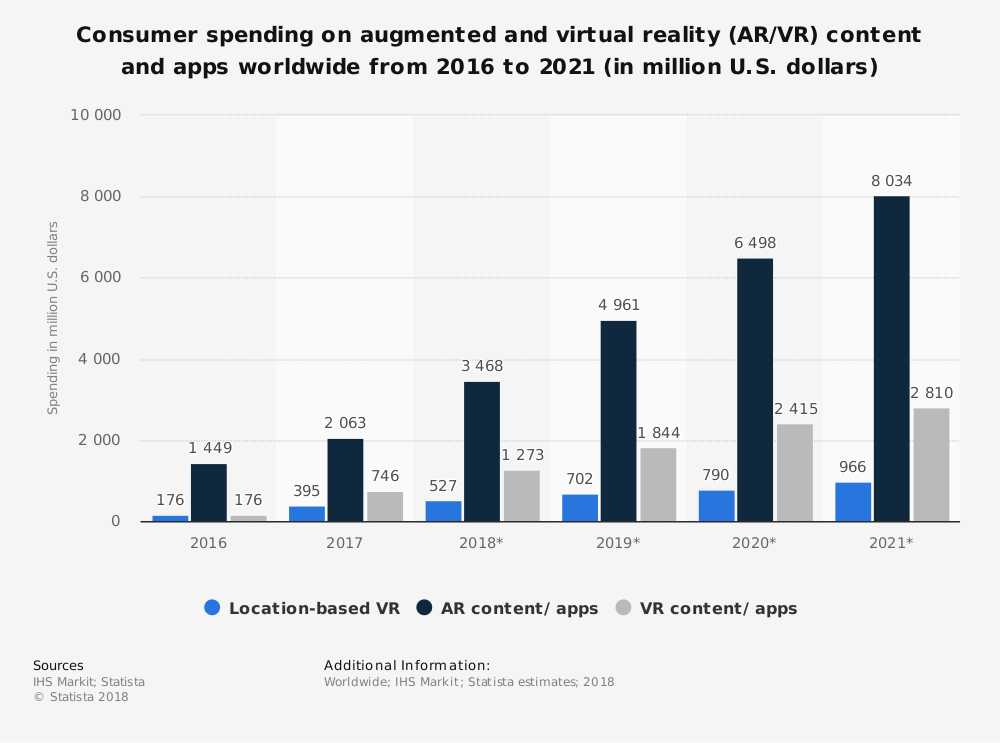
\includegraphics[height=210pt]{ar-vr-consumer-spending}
	\caption{Consumer spending on AR/VR worldwide 2016-2021 \citeyeartitlexamkinline{ar-vr-chart}}
	\label{fig:ar-vr-consumer-spending}
\end{figure}
Literature review is used as a research method for the first part of the thesis. The different literature in the fields of AR,VR and CBRN (Chemical, Biological, Radiological, Nuclear) is reviewed and summarized. The second parth of the thesis is a case study of the practical implementation of a training application. The results will be analyzed by debating the success of the final product and its potential use.
\par
\chapter{\texorpdfstring{Augmented reality and virtual reality}{aug-reality}}
Augmented reality and virtual reality are technologies that offer a different view and experience to the physical world. They leverage similar kinds of technology and both aim to provide an enhanced and enriched experience to the user. Both technologies are a part of the general area of mixed reality \Cref{fig:reality-virtuality}. However they have different goals and are essentially different in terms of user experience.

\begin{figure}[H]
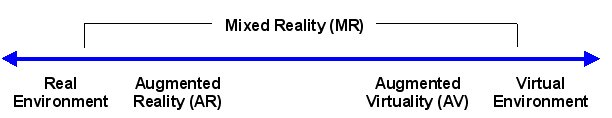
\includegraphics[width=\textwidth]{Virtuality_Continuum_2}
\caption{Reality-Virtuality Continuum (Paul Milgram et al. 2007)}
\label{fig:reality-virtuality}
\end{figure}

\section{Augmented reality}%ref http://kjcomps.6te.net/upload/paper1%20.pdf
Augmented reality (AR) can be described as the technology that bridges reality with virtual environments. Real life objects are transformed or replaced with virtual equivalents. Information can be added or removed to the real environment. Key aspects of AR are the ability to run in real time, be interactive, three dimensional and combine real with virtual information \Cref{fig:ar-application}. AR is most commonly used with the sense of sight, but it can potentially be used with other senses such as hearing, touch, smell, taste, temperature etc. AR can be considered as the next step in graphical user interfaces' (GUI) evolution \citeyearpar{prototyping-ar}. Its current state is comparable to command line interfaces and 2d interfaces in the 1980's and 1990's. It is a vision of future computing and a field that is under research.
\begin{figure}[H]
	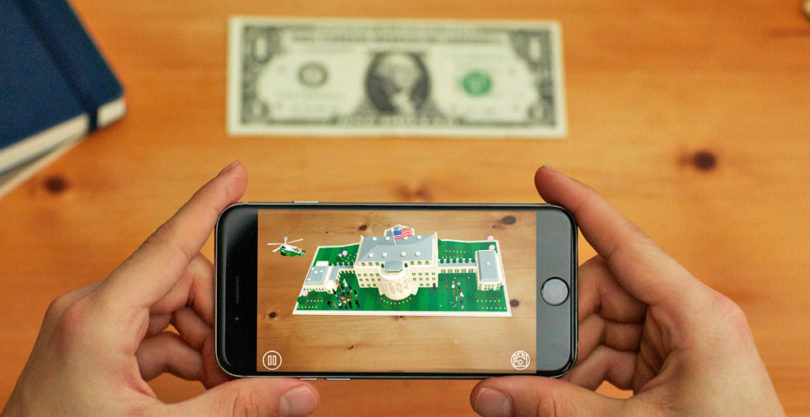
\includegraphics[width=\textwidth]{ar-application}
	\caption{Mobile augmented reality application \citeyearpar{ar-application-whitehouse}}
	\label{fig:ar-application}
\end{figure}
\par
Augmented reality has higher technological requirements compared to VR which has lead to the slower maturity of AR. AR enabling technologies have been developed throughout the history of which the Optical see-through has become the most popular (Microsoft HoloLens, Google Glass, Intel's Vaunt). Optical see-through is achieved by using opaque displays on which virtual overlays can be rendered. The resolution of the real world is left intact as it passes through the screen. Benefits of this approach include power fail safety, which allows users to still see the real world even during a power outage, cheaper production costs of the used displays, no parallax effect that irritates the user's eyes. Disadvantages are the reduced visibility and brightness through the opaque lenses, limitation of the field-of-view, requirement of additional tracking sensors such as cameras, gyroscopes and accelerometers. Due to the lack of maturity of other AR enabling technologies only Optical see-through techniques will be considered throughout this work. \citep{vrjournal}
\subsection{AR for training and education}%ref https://files.eric.ed.gov/fulltext/ED510220.pdf
Augmented reality provides new paths to conveying information. Learning experiences are more contextual by connecting and embedding information with the real world in real time. These approaches are already utilised by Boeing. 
Mechanics in the company use AR goggles that aid repairs with embedded textual instructions, 
illustrate different steps of the repair and help users identify the required tools for a repair. 
Consequently training resources are reduced and transfer of information between workers is greatly 
improved. \citep{horizon-report}
\par
Learning through doing is another approach in which AR shines. Mistakes and errors made during the learning
experience have no real consequences. This provides for more authentic learning experiences which cannot be
achieved easily or cost effectively otherwise. \citep{augmented-reality}
\subsection{AR Challenges}
% As most developing technologies AR has many challenges that need to be overcome or improved. The requirements of the AR framework
% are directly related to those challenges.
An AR framework has basic requirements to accomplish a combination of the real and virtual world.
The four main requirements are sensing, tracking, interaction and displaying \Cref{fig:ar-framework}. Sensing refers to
capturing environment events and recognising markers or other objects of interest. Tracking handles updating the
viewing direction and position of the user relative to the real world. Tracking is an important component
of AR as even a slight tracking error can cause misalignment between the virtual and real world objects. \citep{ar-design} 
Registration refers to how the digital information is delivered to the user. Registration can be achieved
through different methods for different senses: videos, audio, haptic feedback, scent, etc.
\begin{figure}[H]
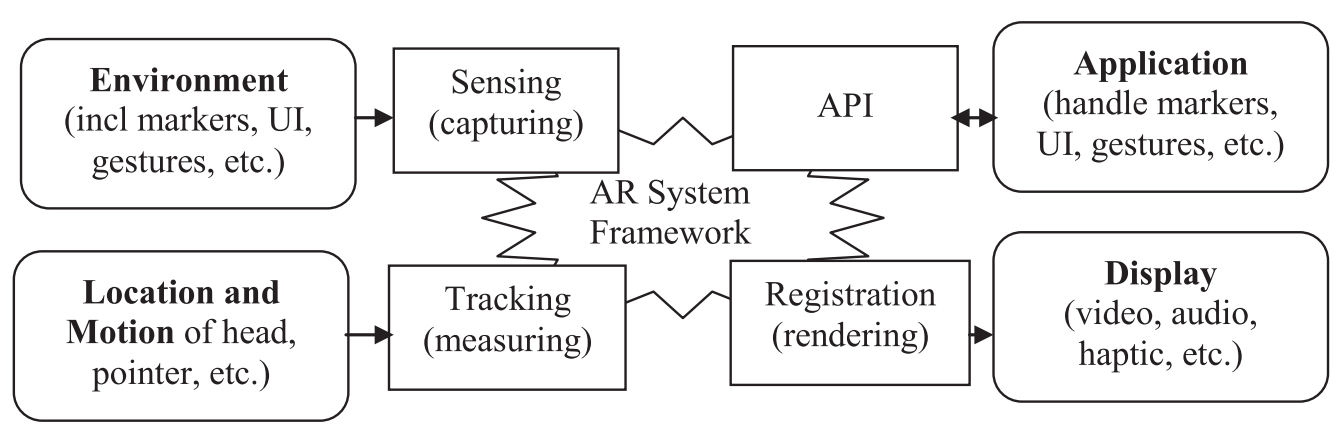
\includegraphics[width=\textwidth]{ar-framework}
\caption{Augmented reality framework \citep{vrjournal}}
\label{fig:ar-framework}
\end{figure}
As most developing technologies AR, has many challenges that need to be overcome before it can be widely adopted.
The challenges of AR arise from the framework requirements, and they can be divided into five groups \Cref{fig:ar-challenges}.
\begin{figure}[H]
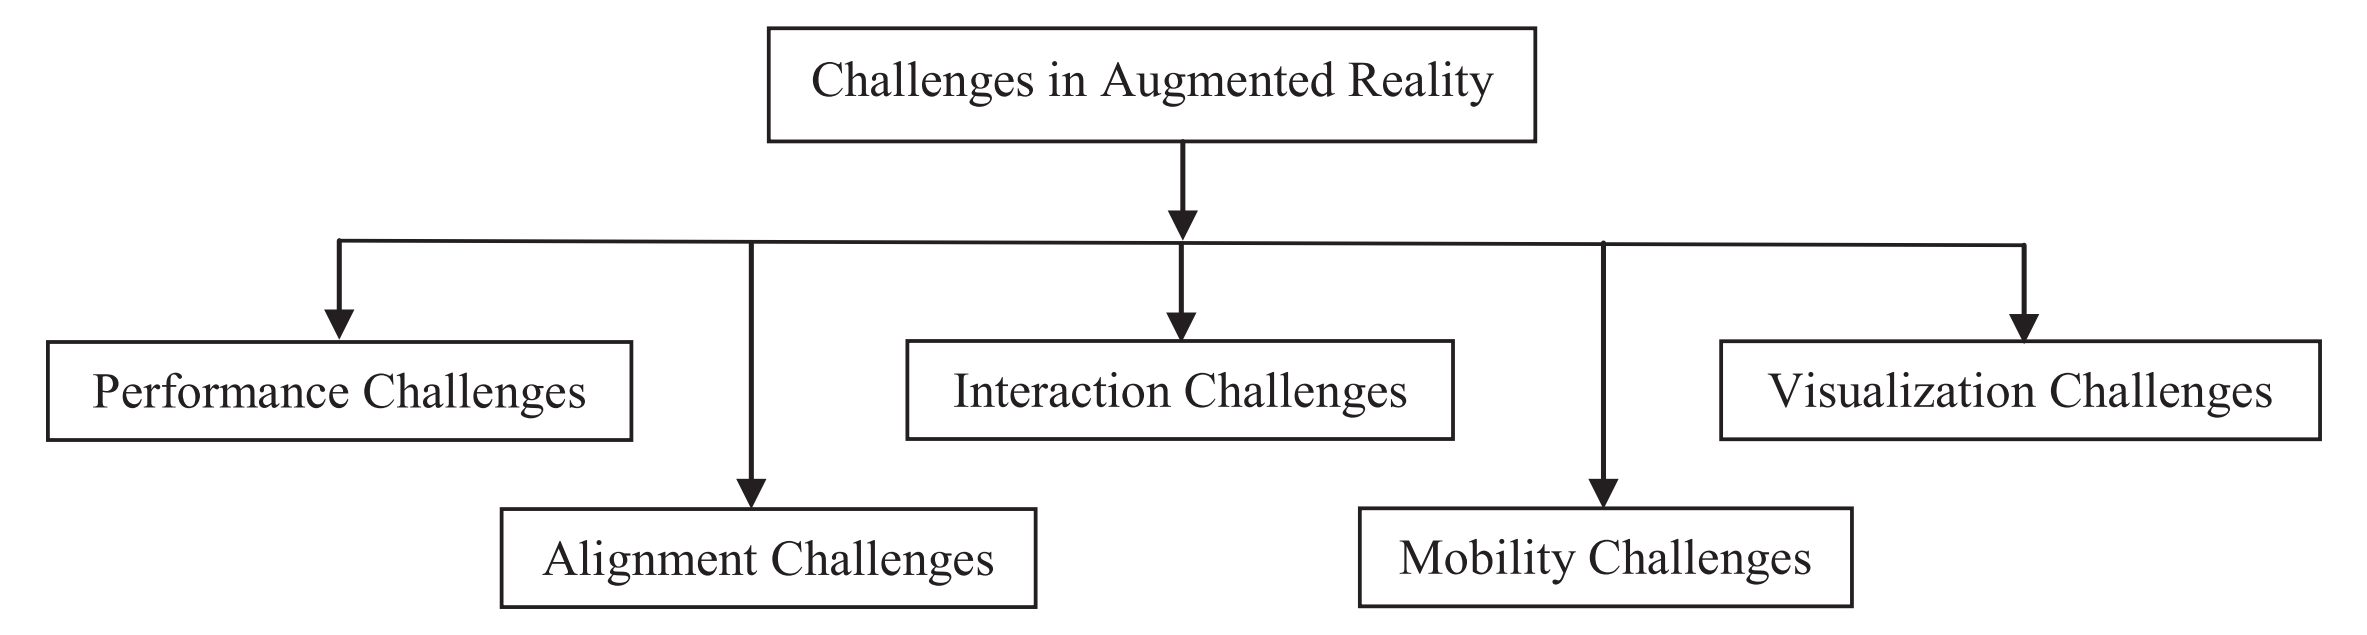
\includegraphics[width=\textwidth]{ar-challenges}
\caption{Augmented reality challenges \citep{Acta-Graphica}}
\label{fig:ar-challenges}
\end{figure}
Performance challenges arise from the need of real time processing. AR tasks such as marker detection
and virtual object rendering are computationally intensive, and this slows down performance.
Alignment challenges come from the complexity of tracking the users movement and registration of real
life objects. Any errors in these methods can cause misalignment between the rendered objects and
real view.\par
Interaction challenges are concerned with the interaction between users and virtual or real objects.
User interfaces need to be intuitive and unobstructive for the best experience. Mobility challenges refer
to the need of portability for AR systems.
\\
\section{Virtual reality}
Virtual reality (VR) in the broadest sense is the method or technology of substituting a physical environment with a virtually perceived environment. The Oxford dictionary gives a more detailed definition: 
''The computer-generated simulation of a three-dimensional image or environment that can be interacted with in a seemingly real or physical way by a person using special electronic equipment, such as a helmet with a screen inside or gloves fitted with sensors''.
This is typically achieved by using an HMD (Head mount display) with integrated motion tracking and a built-in or external rendering unit.
The requirements of VR are similar to those of AR with the exclusion of environment sensing \Cref{fig:ar-framework}. The virtual environment
is entirely digitally constructed, thus eliminating the need for sensing as all environmental events are native to the system. This is achieved with a VR headset that has different views for each eye, accomplishing depth perception \Cref{fig:htc-vive-pro-headset}.
\begin{figure}[H]
	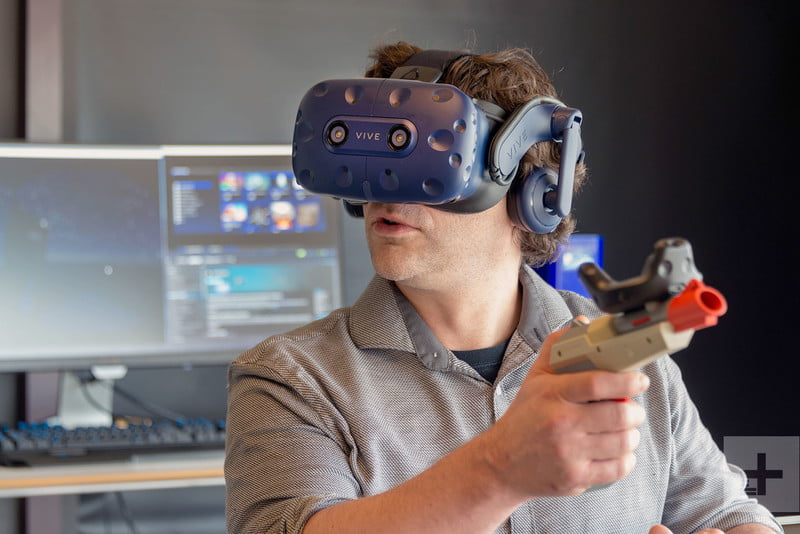
\includegraphics[width=\textwidth]{htc-vive-pro-headset}
	\caption{HTC VIVE Pro headset \citeyearpar{htc-vive-pro-review}}
	\label{fig:htc-vive-pro-headset}
\end{figure}
\par
Interaction with the environment isn't necessary for a VR experience, but it increases the possibilities and usability of a VR system.
Different approaches to user interaction offer various degrees of immersion and limitations. Motion tracked controllers, hand motion tracking gloves, pointer centered to the viewport, headset location tracking in 3D space and sekeletal motion tracking are common approaches.
\subsection{VR challenges}
Virtual reality challenges can be categorized in the same way as AR challenges \Cref{fig:ar-challenges}.
Performance is a very important factor in keeping the VR experience immersive for a prolonged period of time.
High resolution picture rendering at a high framerate in real-time is taxing even for the highest end of current GPUs. 
Lower framerate or lower resolution picture can cause dizziness, eye tiredeness and overall dissatisfaction. Alignment challenges arise from the difficulty of tracking in real-time.
Users' view, location or controllers can become misaligned with the virtual environment, breaking the immersion and interactability.
Interaction challenges come from the current hardware limitations on interacting. Tactile feedback, hand interaction and free movement in the 3D space are all possible techniques individually, but combining them at the same time is not yet achievable.
\par %(Interrante et al., 2008; Mohler et al., 2010; Phillips et al., 2010).
Mobility challenges arise from the need of portability for VR platforms. Common solutions
rely on tethering to a machine that handles the rendering and power supply. However, portable VR backpacks and headsets are starting to emerge. A notable example of which is the HP VR backpack \citeyeartitlexamkinline{hp-vrbackpack}.
Visualization can be difficult due to the complexity of the physical world. Keeping proportions, lighting, textures, view depth, field of vision and other visiual perception aspects can be challenging.
\subsection{VR for education and training}
Virtual reality has many prospects for use in education. Learning can be promoted by interacting with objects and the environment in a virtual world. 
Similarly self-paced exploration can improve the users' ability to understand a given topic.
%reference VR Collaborative learning
Learning through doing is even more prominent with VR than AR. Scenarios that are hard or impossible to create with traditional approaches can be executed in a virtual environment for the fraction of the cost.
Users that are physically apart can be in the same virtual environment.
Professors or specialists don't need to travel to remote locations to train people.
\section{Hybrid approaches}
\par
Hybrid approaches to VR and AR can be used to create solutions that overcome imposed drawbacks by the techologies. These approaches include using physical objects or combining different sensors.
Such a drawback for VR is the lack of tactile feedback or realistic hand interaction with the environment. This becomes a problem when training pilots as they get accustomed to the feel of the virtual environment and are unable to perform tasks as quickly in the real environment.
Feedback from the cockpit instruments is essential as well as the ability to use them with peripheral vision.
One solution to this problem has been developed by NLR (Royal Netherlands aerospace centre) with the use of a hybrid approach.
IR depth sensors and a camera feed are used to map the pilots' hands in the virtual cockpit. Mockups of the flight instruments are 3D printed and are mapped to the virtual environment with tracking markers.
This allows for a much more natural feel of the flight instruments and offers better training results. \citep{nlr-vr}
\\
\section{Simulation training}
Simulation training is the process of using a controlled but competitive virtual environment to acquire real world skills. By implication the environment is an imitation of a real environment and the training is an imitiation of a real-life process. The process can also be recorded, analyzed and scored based on the results of the trainee. \citep{enterprise-simulation}
\par
Simulation training has been used for decades in the fields of  healthcare, military and aviation \citeyeartitlexamkinline{simulation-training-history} and several benefits have been observed. The simulated environment is safe and secure, which allows trainees to practice and gain experience with the risk of mistakes being eliminated. Teamwork behaviours such as communication, collaboration, team leading can be improved in practice. Insight into the trainee's behaviour can also be obtained by recording and analyzing training sessions. \citep{medical-sim-training}
\par
In the military education field simulations are widely adopted. Strategy and tactics games have been used for officer training by the US Army forces. USA Command and General Staff College also uses a turn-based strategy game for their Crops-level operations course. Skill and Team Building has also has benefited from simulation training by using "first person shooter" games. Flight simulation is clearly one of the biggest beneficiary of simulation training according to an extensive study conducted by the US Navy. Higher scores were obtained by students who used the simulation product prior to the early flight training. \citep{games-sim-mil}
\par
With so many examples of good simulation training being effective and widely adopted it is possible to conclude that the SAS civil and military defense system can also benefit from such training.
\\
\chapter{\texorpdfstring{Project use case}{proj-use-case}}
Observis Oy is developing a product for situational awareness in different environments called ObSAS. This product is a software system running on multiple devices with multiple purposes. The product consists of several software packages with different purposes and providing different features. Depending on the project the required packages are selected and used. One main package is the low level software that communicates with various sensors and devices, such as chemical detectors, radiation sensors, biological detectors. Another package is the server software which summarizes the data and handles automatic actions. User software package allows users to interact
with all components of the system. The software packages can be integrated into varying environments and the final complexity of the product installation can also vary. Additionally required hardware and hardware installation support can be provided. Software support and maintenance can also be provided.
\par
The end use for the product is usually civil defence or shelter management. High reliability and availability are crucial requirements for the final product as human lives can be put in danger by improper operation of the software or misuse by the users. Training is necessary to ensure proper use of the software and 
other components of the situational awareness system. So far traditional training approaches have been used, such as powerpoint slides including pictures of the software, textual description of individual components and narration from the training personnel.
\par
\section{Current training approach}
Current training is done on customers' premises in two parts - theoretical and practical. The theoretical part takes place in a classroom with teaching tools such as whiteboard and projector provided by the customer. A group of around 20 people is trained during the theoretical part with the use of powerpoint slides containing screen captures of the software. Additionally, the software enabled in simulation mode is displayed and used in front of the trainees. Devices such as laptops, external hard drives and cameras are not allowed during the training to avoid redistribution of confidential information.
\par
The second part of the training involves practical use of the system. One example project in which practical training was used is the Sassi case. In the Sassi project case the training takes place inside a reconnaissance vehicle with a group of up to four people. Real life devices are used with the software. Test sources are used to trigger devices' alarms and cable disconnection is used to test failure states.
 Test sources or simulants are compounds or biological samples that are used to verify proper operation of the detection devices. For chemical detection devices such simulants can be samples of acetone, ethanol, MSAL, acetic acid for Toxic Industrial Chemicals(TICs) and DMMP, DIMP for Chemical Warfare Agents(CWAs). The chemical simulants are provided at the air intake of the detection device and the time to alarm from exposure is observed. The time it takes for the device to clear out after the initial exposure is also monitored. These intervals can indicate if a device is operating correctly. The trainees are familiarised with these basic operations of the devices. More advanced operations such as creating reports, marking contamination areas and changing air intake directions are also practiced.
\par%switched to past perfect, not sure why, a bit inconsistent?
Feedback from the customer in the Sassi project has been positive, although there have been complaints from the trainees about the translation of the materials, but still overall positive feedback has been received. According to Jukka Härkönen(an employee from Observis who conducts the training) the trainees with better English language skills have managed to attain more knowledge from the training. Trainees who were familiar with a previous version of the software have had no problems adjusting to the differences in the new version of the product. Some trainees however have not been able to fully prepare for the use of the software and require further internal training conducted by the customer.
\section{Future goals}
Regardless of the good customer feedback there is room for improvement in the training. Streamlining the training can reduce the time required to create training materials and the amount of staff needed to conduct the training. Another future goal of the training is to be able to experience more lifelike situations and more complex scenarios resulting in better preparedness for critical situations. Misunderstanding caused by a language barrier is something that should be avoided in future training.
\par
Innovation in every aspect of the product is welcomed from the customers. The market has been stagnant and competing companies have been refusing to innovate due to the various risks involved with doing so. Observis is willing to take those risks to set itself apart. A survey and analysis of virtual reality technologies interests the company.
\par
\section{Defining the application specifications and requirements}
A particularly sophisticated requirement of the system is the maintenance procedure. Measurement devices and sensors require periodic maintenance and inspection to remain in good operating condition. Negligence of maintenance can lead to faulty readings over time, device breakdown or even failure to recognise threats. The maintenance involves physical interaction with the measurement device that is guided by an instructional document. Software use is also required during the procedure to mark used parts and add additional notes. It is not possible to practice all maintenance procedures during training because of the time constraint. Consumables such as filters, batteries, tubings are often needed for the maintenance which can increase the cost of training. For the above-mentioned reasons implementing a training scenario that involves conducting maintenance in a mixed reality environment would be of great benefit.
\par
One particular device that requires maintenance is Environics ChemProDM. The device is a Chemical Warfare Agents (CWA) and Toxic Industrial Chemicals (TIC) detector that is targeted for vehicle use \Cref{fig:chemprodm}. Typical installation includes two modules: ChemProDM detector and Remote Alarm Unit. A maintenance training scenario for this device is a great candidate for a mixed reality application. Initial installation and testing are also interesting use cases that can benefit from a training application.
\begin{figure}[H]
	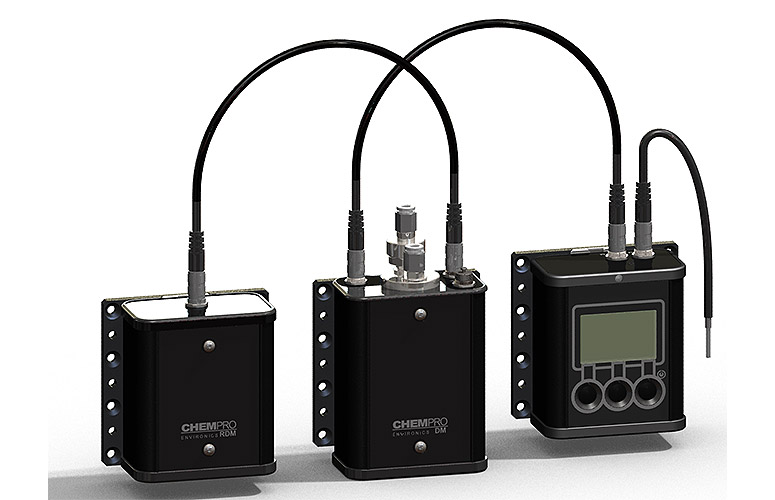
\includegraphics[width=\textwidth]{chemprodm}
	\caption{ChemProDM and modules \citeyearpar{environics-chemprodm}}
	\label{fig:chemprodm}
\end{figure}
\par
Other devices included in ObSAS are the Thermo SVG2 radiation sensor, Meteo IRDAM MAWS 5060 weather sensor and the Infinicon Hapsite ER chemical analyzer. Basic knowledge of these devices is a great benefit when using the system. However, it is not required of the users. The user can be familiarized with the devices during training. The knowledge attained can be helpful if on field repairs are required.
\par
\section{CBRNe defense}
CBRNe is an acronym for Chemical, Biological, Radiological, Nuclear and Explosives. CBRNe defense is the field of detecting, reducing the impact of or avoiding the threats of CBRNe agents. In recent years the threat of CBRNe attacks has increased due to technological development and increased willingness of terrorists to obtain and use such agents. \citep{crowd-behavior}
\par
A motivation for CBRNe defense is the amount of casualties taken by CBRNe threats all around the world all the time. Such incidents are covered bi-monthly in the CBRNeWORLD magazine and their numbers are not decreasing \citeyearpar{cbrne-world}. The industry in this field aims to provide solutions that prevent or reduce the impact of CBRN incidents and attacks. Market share of the field has been growing steadily and the forecast is of continuous growth for the future years to come according to Visiongain's market report \citeyeartitlexamkinline{cbrn-market-share}.
\par
ObSAS provides possibilites for early detection and prevention of CBRN attacks. Gathering as much information possible about the attack can help with planning impact reduction and prevention strategies. ObSAS allows for the gathering and analysis of such data: chemical threat identification, air spectrum analysis, radiation measurement, geographical location and meteorological conditions. A vehicle with an ObSAS installation can safely cover and inspect a large area. Communication channels can be used to share and collect data from various CBRN sources. A more clear picture of threats can be established that way.\par
The CBRN field also encompasses considerations such as decontaminating equipment and clothes, medicine administration, using protective equipment and detection devices require training and practice. Databases providing instructions on what actions to take depending on the threat are often available in CBRN software. The use of such databases also benefits from prior training.
\section{Comparing VR and AR in the project context}
AR and VR differ not only in hardware but also in software development kits. It is rarely the case that an application written for one of the platforms can be seamlessly ported to the other. Therefore the two technologies need to be compared in regards to the current project. To keep the scope of this thesis narrow a single technology will be used to implement a training application.
\par
AR hardware such as goggles, glasses and headsets are generally very portable and self-contained. This makes it easy to transport the required hardware during training or installation tirps. The initial setup of the training environment could be more tedious with AR. If real life devices need to be tracked, markers have to be placed and calibrated. As seen from the specification sheet on the Microsoft store \citeyeartitlexamkinline{hololens-specs}, the HoloLens have narrow field of view, smaller color space, low luminosity and lower computing power compared to VR headsets. This can result is reduced immersion and engagement with the virtual environment. Another downside is the inability to emulate real life scenarios such as being inside a moving vehicle or simulating an environment that is completely different from the one the user is in. For example it is impossible to simulate night missions if the user is in a brightly lit room. For these reasons AR is restricted by the environment it is being experienced in.
\par
The easability of use of AR headsets is one important benefit. While VR headsets require a tether cable, external computer and even base stations in some cases, AR headsets can be used as they are, independently. 3D modelling isn't as big of a requirement compared to VR as it is enough to create models only of the objects the user interacts with, not the full environment the user is in. This can reduce development time significantly.
\par
VR shines in implementing a completely independant environment. The only limit to what can be recreated is imposed by the hardware performance and development time and skills. VR allows for spectating and recording users' interaction with the environment. This can be used to analyze their experience and improve the software further. Giving suggestions and guiding during the training is also possible. A multi-user environment is also possible and trainees and teachers can be in the same environment even if they're physically far apart.
\par
Price difference is very small between VR and AR if the most advanced frameworks are being considered. An AR headset with the development pack such as Microsoft HoloLens is priced at 3000\$ on the Microsoft store \citeyeartitlexamkinline{hololens-price}. And a VR headset such as HTC Vive Pro is priced at 1500\euro\ on the official VIVE store \citeyeartitlexamkinline{htc-vive-pro} with VR capable laptops priced starting from 1500\euro. Similarly prices of development kit licenses are not far apart either. This makes the decision between the two based entirely on the features they provide, driven by the requirements of the use case they're aimed for.
\par
\section{Selection of mixed reality framework}
The main benefit of AR over VR in this project is the portability and ease of use it offers. In terms of what training can be implemented VR offers a lot more possibilities. Battery limitations are also reduced or avoided which enables long training sessions. Good multiplayer support and additional peripherals(such as gloves and controllers) are in favor of VR too. The portability of AR is not a crucial feature for this project and the usability it offers over VR are not sufficient enough to place AR as a more suitable platform in this project. A conclusion to this chapter is that a VR framework is a more suitable choice in the context of creating a training application for the ObSAS system.
\par
\chapter{\texorpdfstring{Project definition}{proj-def}}
This chapter will describe the virtual application in more detail and outline the different technologies used in the implementation. Concepts such as 3D computer graphics, 3D modelling, game engine and tracking will be defined. Source code used in the development of the application will be provided and explained.
\par
\section{Researching VR hardware and software}
The most notable VR headsets available on the market are Occulus Rift and the successor to HTC VIVE, the HTC VIVE Pro. Widest software and peripheral support is offered to these headsets, so other options would not be considered. The main difference between the two is that HTC VIVE Pro has higher screen resolution and pixel density \Cref{fig:comparison-table}. Occulust Rift has lighter controllers, but requires at least 3 or even 4 sensors in some cases for decent room tracking. In contrast HTC VIVE Pro offers a wider tracking area with just 2 tracking sensors as pointed out by WindowsCentral VIVE Pro vs Occulus Rift article \citeyeartitlexamkinline{vive-vs-rift}. Both options provide the required features, but HTC VIVE Pro is more suitable and offers more because of the better graphics. 
\begin{table}[H]
	\begin{tabular}{|l|l|l|}
	\hline
	\textbf{Category}   & \textbf{HTC VIVE Pro}                                               & \textbf{Occulus Rift}                                                \\ \hline 
	\textbf{Display}    & Dual Amoled 3.5                                                   & Dual Amoled 3.54"                                                    \\ \hline
	\textbf{Resolution} & 1440x1600(2880x 1600)                                               & 1080x1200(2160x1200)                                                 \\ \hline
	\textbf{PPI}        & 615                                                                 & 461                                                                  \\ \hline
	\textbf{FOV}        & 110 degrees                                                         & 110 degrees                                                          \\ \hline
	\textbf{FOV}        & 90Hz                                                                & 90Hz                                                                 \\ \hline
	\textbf{Connection} & \begin{tabular}[c]{@{}l@{}}USB-C 3.0\\ DisplayPort 1.2\end{tabular} & \begin{tabular}[c]{@{}l@{}}HDMI\\ USB-A 2.0\\ USB-A 3.0\end{tabular} \\ \hline
	\end{tabular}
	\caption{HTC VIVE Pro vs Occulus Rift specs}
	\label{fig:comparison-table}
\end{table}
VR hand and finger tracking is a great addition to the immersion of the VR experience. More intuitive interaction with the virtual environment is possible. Many gloves are available as prototypes on the market. Some feature resistive finger feedback and texture and shape simulation like the VRGluv \citeyeartitlexamkinline{vrgluv}. A large portion of such gloves are in the prototyping stage and can only be preordered. The Noitom hi5 gloves however are available as a purchasable product, even though they're missing the aforementioned features.
\par
These gloves achieve full finger tracking by using 9 inertial measurement units on each glove. The VR headset controllers are strapped on the gloves to provide absolute tracking \Cref{fig:vr-glove}. Vibration feedback is also supported by the hardware and software API as documented by Noitom on their product website \citeyeartitlexamkinline{hi5-vr-glove}.
\begin{figure}[H]
	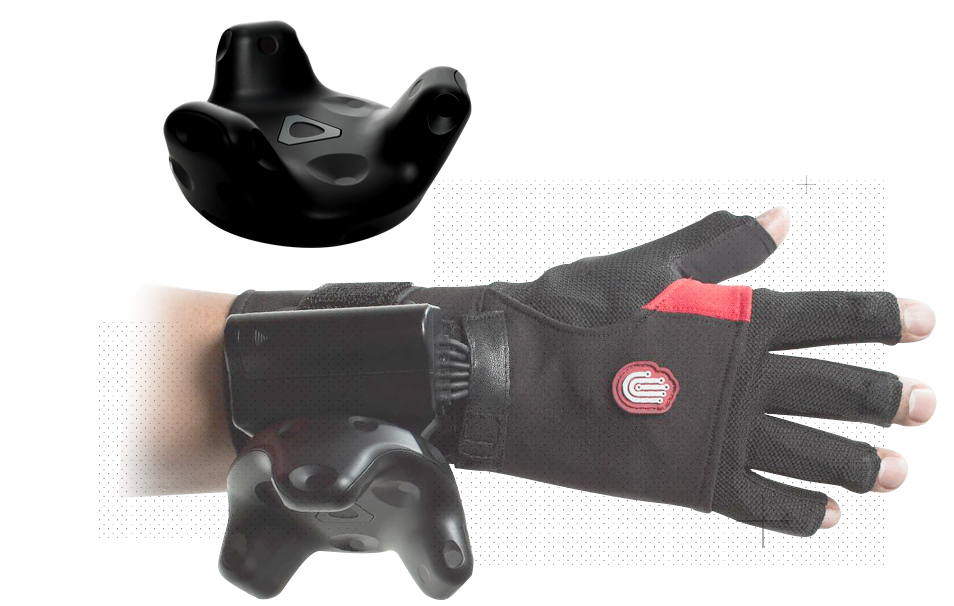
\includegraphics[height=210pt]{vr-glove2}
	\caption{Noitom HI5 VR glove with VIVE trackers \citeyeartitlexamkinline{hi5-vr-glove}}
	\label{fig:vr-glove}
\end{figure}
\par
The Noitom hi5 gloves are compatible with HTC VIVE Pro and offer SDKs for the most popular game engines (Unreal Engine and Unity). These gloves will be used in the project to achieve better immersion and quality of training.
\section{Game engines}
A game engine is a software framework aimed at simplifying and streamlining the production of games. At the core it provides a 3D or 2D rendering engine, generic physics engine, sound, animation and other features that assist game creation but do not directly specify the game's behavior. If used successfully a game engine can produce a higher quality game with less resources and in less time. An engine isn't required to build applications as all the features can be implemented from the ground up without the need for reusability or modularity, but that takes significantly more resources than using already existing tools. \citep{game-engines}
\par
Despite having the name game engine, such engines have many other applications besides making games. They can be used for pretty much any graphical application. Simulation applications, training applications, VR and AR applications of any kind, presentations, cinematography can all benefit from using a game engine. Using a game engine is suitable for this project because of the time constraint and limited resources available. 
\par
One popular game engine is Unreal Engine, created by Epic Games Inc. It is widely adopted and it offers a large selection of plugins, addons, libraries and assets that aid development. Unreal Engine supports various VR and AR platforms including HTC VIVE Pro and Hi5 vr gloves. This engine will be used to develop the training application.
\section{Application Objectives}
The application objectives can be defined as a set of actions that the user needs to complete in a certain order. Using objectives helps quantifying the training progress and give guidance to the user at the same time. Having structured objectives also helps motivate users to continue interacting with the software. \citep{goal-oriented-games}
\par
Defining the application objectives also helps the development process. In the context of this 3D application the required assets can be inferred from the application objectives. These assets include 3D models the user interacts with, sound effects, written instructions, 2D graphics, background environment models. Gathering a list of these assets and their description is necessary for outsourcing the 3D modelling work or sound effect composition. Such topics are out of the scope of this thesis, therefore the production process of the used assets will not be covered.
\par
The training will take place inside a virtual environment. This virtual environment consists of the interior of a vehicle, all detection devices, computational devices, power distrubition and sampling system. The first objective is to explore the vehicle and get acquainted with the environment. The second objective is to check whether all connectors are plugged at the correct places and inspect all cables for visual signs of wear. The third objective is to power up the entire system and wait for baseline acquirement of all detection devices. Once that is complete the next objective is to begin chemical detection tests with simulants. If the simulant causes a chemical alarm the user will also be required to acknowledge that alarm and print a report.
\par
The next objective is to test radio-nuclear detection by using a sample of radioactive rock ore. Again if an alarm is prompted the same actions need to be repeated. Afterwards biological detection is tested with simulants. The last objective is to assure that the system has reached baseline operation again and then shut it down.
\par
With the list of objectives defined in Figure \ref{fig:objectives-table} it is possible to create a list of the required 3D models. This list can be used to request modelling work, which will be done internally at Observis Oy. Obtaining 3D models of the detection devices proved to be difficult as companies are not willing to provide these without any ongoing projects related to the devices.
\par
All the objectives take place in a relatively small area which means they can be a part of a single Level. Unreal Engine Levels are explained in the next section.
\begin{table}[H]
	\centering
	\begin{tabular}{@{} |M{0.45cm}|p{2.5cm}|p{6.5cm}|M{2.4cm} |@{}}
	\hline
	\textbf{\#} & \textbf{Description}        & \textbf{Models}                                            & \textbf{Compulsory} \\ \hline
	1           & Explore the vehicle         & Vehicle                                                    & \checkmark          \\ \hline
	2           & Check connections           & Wires, Plugs, Sockets, Power/Junction box                  & \checkmark          \\ \hline
	3           & Power up the system         & Power switch, Indication lights, Display and Computer      & \checkmark          \\ \hline
	4           & Chemical simulant testing   & Chemical simulant, Chemical detector, Air sampling box     & \checkmark          \\ \hline
	5           & Chemical Alarm              & Keyboard, Mouse, Laptop/Computer                           &                     \\ \hline
	6           & Radiological testing        & Radiological detector, radioactive sample                  & \checkmark          \\ \hline
	7           & Radiological Alarm          & Keyboard, Mouse, Laptop/Computer                           &                     \\ \hline
	8           & Biological simulant testing & Biological detector, Biological simulant, Air sampling box & \checkmark           \\ \hline
	9           & Biological Alarm            & Keyboard, Mouse, Laptop/Computer                           &                     \\ \hline
	10          & System shutdown             & Power switch, Indication lights, Display and Computer      & \checkmark           \\ \hline
	\end{tabular}
	\caption{List of Objectives and required 3D models}
	\label{fig:objectives-table}
\end{table}
\par
\section{Unreal Engine Level}
Levels are defined in Unreal Engine's documentation as a collection of Static Meshes, Volumes, Blueprints and other entities that the user sees and interacts with \citeyeartitlexamkinline{ue-levels}. They are helpful to organize a project into different virtual locations or chronologically. Levels are treated similarly to other assets in UE. They can be created, loaded and modified from the Content Browser.
\par
The full training takes place inside a virtual vehicle, which can be accomplished by using a single level. UE4 comes with starter content when creating a new project. One level that comes with the VR project template is the MotionControllerMap \Cref{fig:level-ue4-editor}. This level features a VRPawn object which is responsible for the majority of functionalities related to the user. It handles tracking of the Head Mounted Display and syncing camera to it, input from controllers, mapping the controllers' location to static meshes, player positioning in the environment and others.
\begin{figure}[H]
	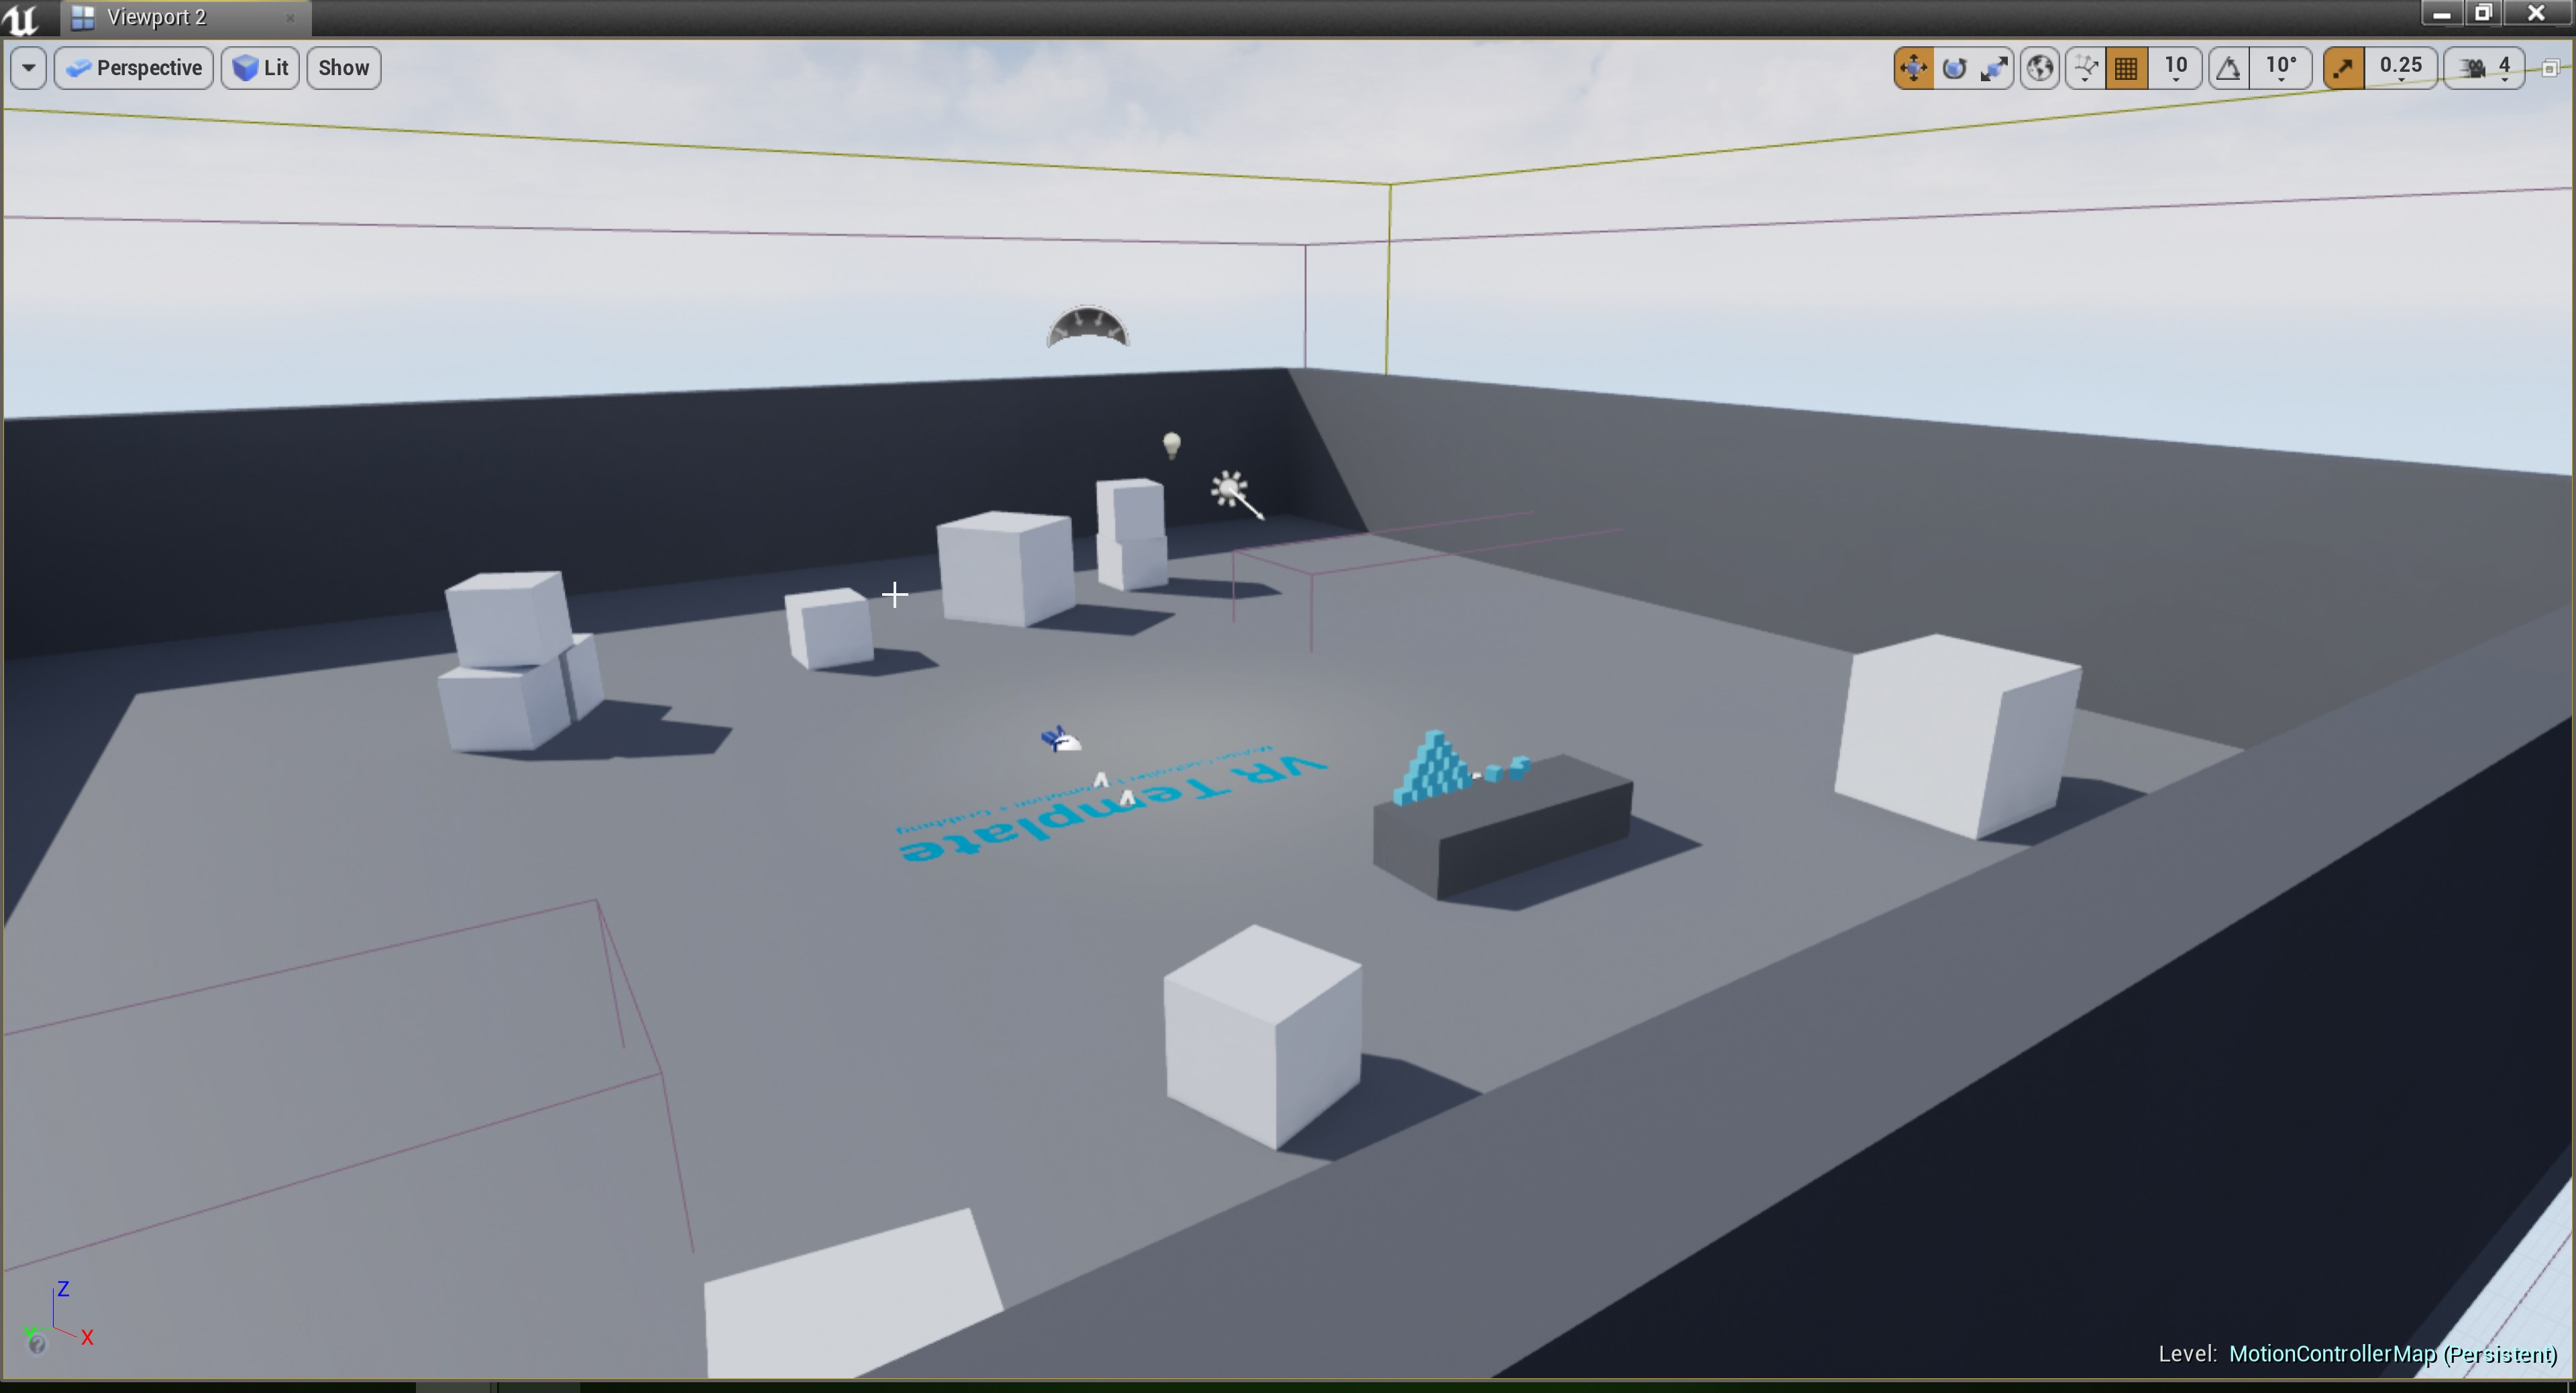
\includegraphics[width=\textwidth]{level-ue4-editor}
	\caption{UE4 MotionControllerMap Level Viewport}
	\label{fig:level-ue4-editor}
\end{figure}
Other objects in this level are the different light entities which include ambient light, point light, sky light and light interaction and postprocessing. This level also comes with several meshes, some of which have simulated physics interaction. And the last type of components in this level are the NavMeshBoundsVolume and NavModifierVolume entities which define what areas in the level the user can walk on.
\par
This starter content level provides all the basic functionalities needed for this project. It can be used as a starting point for the implementation and further extended and modified to contain the full training. In the future more levels can be added for different locations and scenarios.
\subsection{Actors}
Actors are generic Classes in UE that support 3D transformations such as transformation, rotation and scaling. These actors can be created(spawned) and destroyed dynamically while the application is running. They can also be updated dynamically by "ticking", which means that they can be updated with every rendered frame(tick). Another main function of Actors is replication and controlling behaviour of objects in network play(multiplayer). Actors hold different types of objects which are called Components, in a sense Actors are containers for Components. The main types of Components Actors can hold are UActorComponent, USceneComponent, UPrimitiveComponent. UActorComponents have conceptual functionality, they don't exist anywhere in the world. They can be used for example to implement AI functionality, handle user input, saving/loading game progress. USceneComponents are placed in the world and have a location, scale and rotation parameters. UPrimitiveComponents have graphical presentation from a static mesh, particle system, 2D graphics or other primitive assets. Physics, collision and overlap settings are available for these components.  
\par
Some examples of actors in this project are StaticMeshActors of the different detection devices, CameraActor responsible for what the player sees, PlayerStartActor that defines the player starting point. Actors are also hierarchical with one Root Actor having nested Actors on several levels. Controlling the actors can be done with gameplay code written in C++ or with blueprints. \citeyeartitlexamk{ue-actors}
\subsection{Blueprints}
Blueprint is a visual scripting tool in Unreal Engine that offers the full range of development tools and concepts generally available only to programmers. A node-based visual interface is used in which different Events, Nodes, Functions and Variables are connected with Wires \Cref{fig:ue-blueprint-tool}. These connections can define complex gameplay logic by combining and chaning multiple simple operations and creating conditional logic. Objects created with this visual tool are referred to as Blueprints. \citeyeartitlexamk{ue-blueprints}
\begin{figure}[H]
	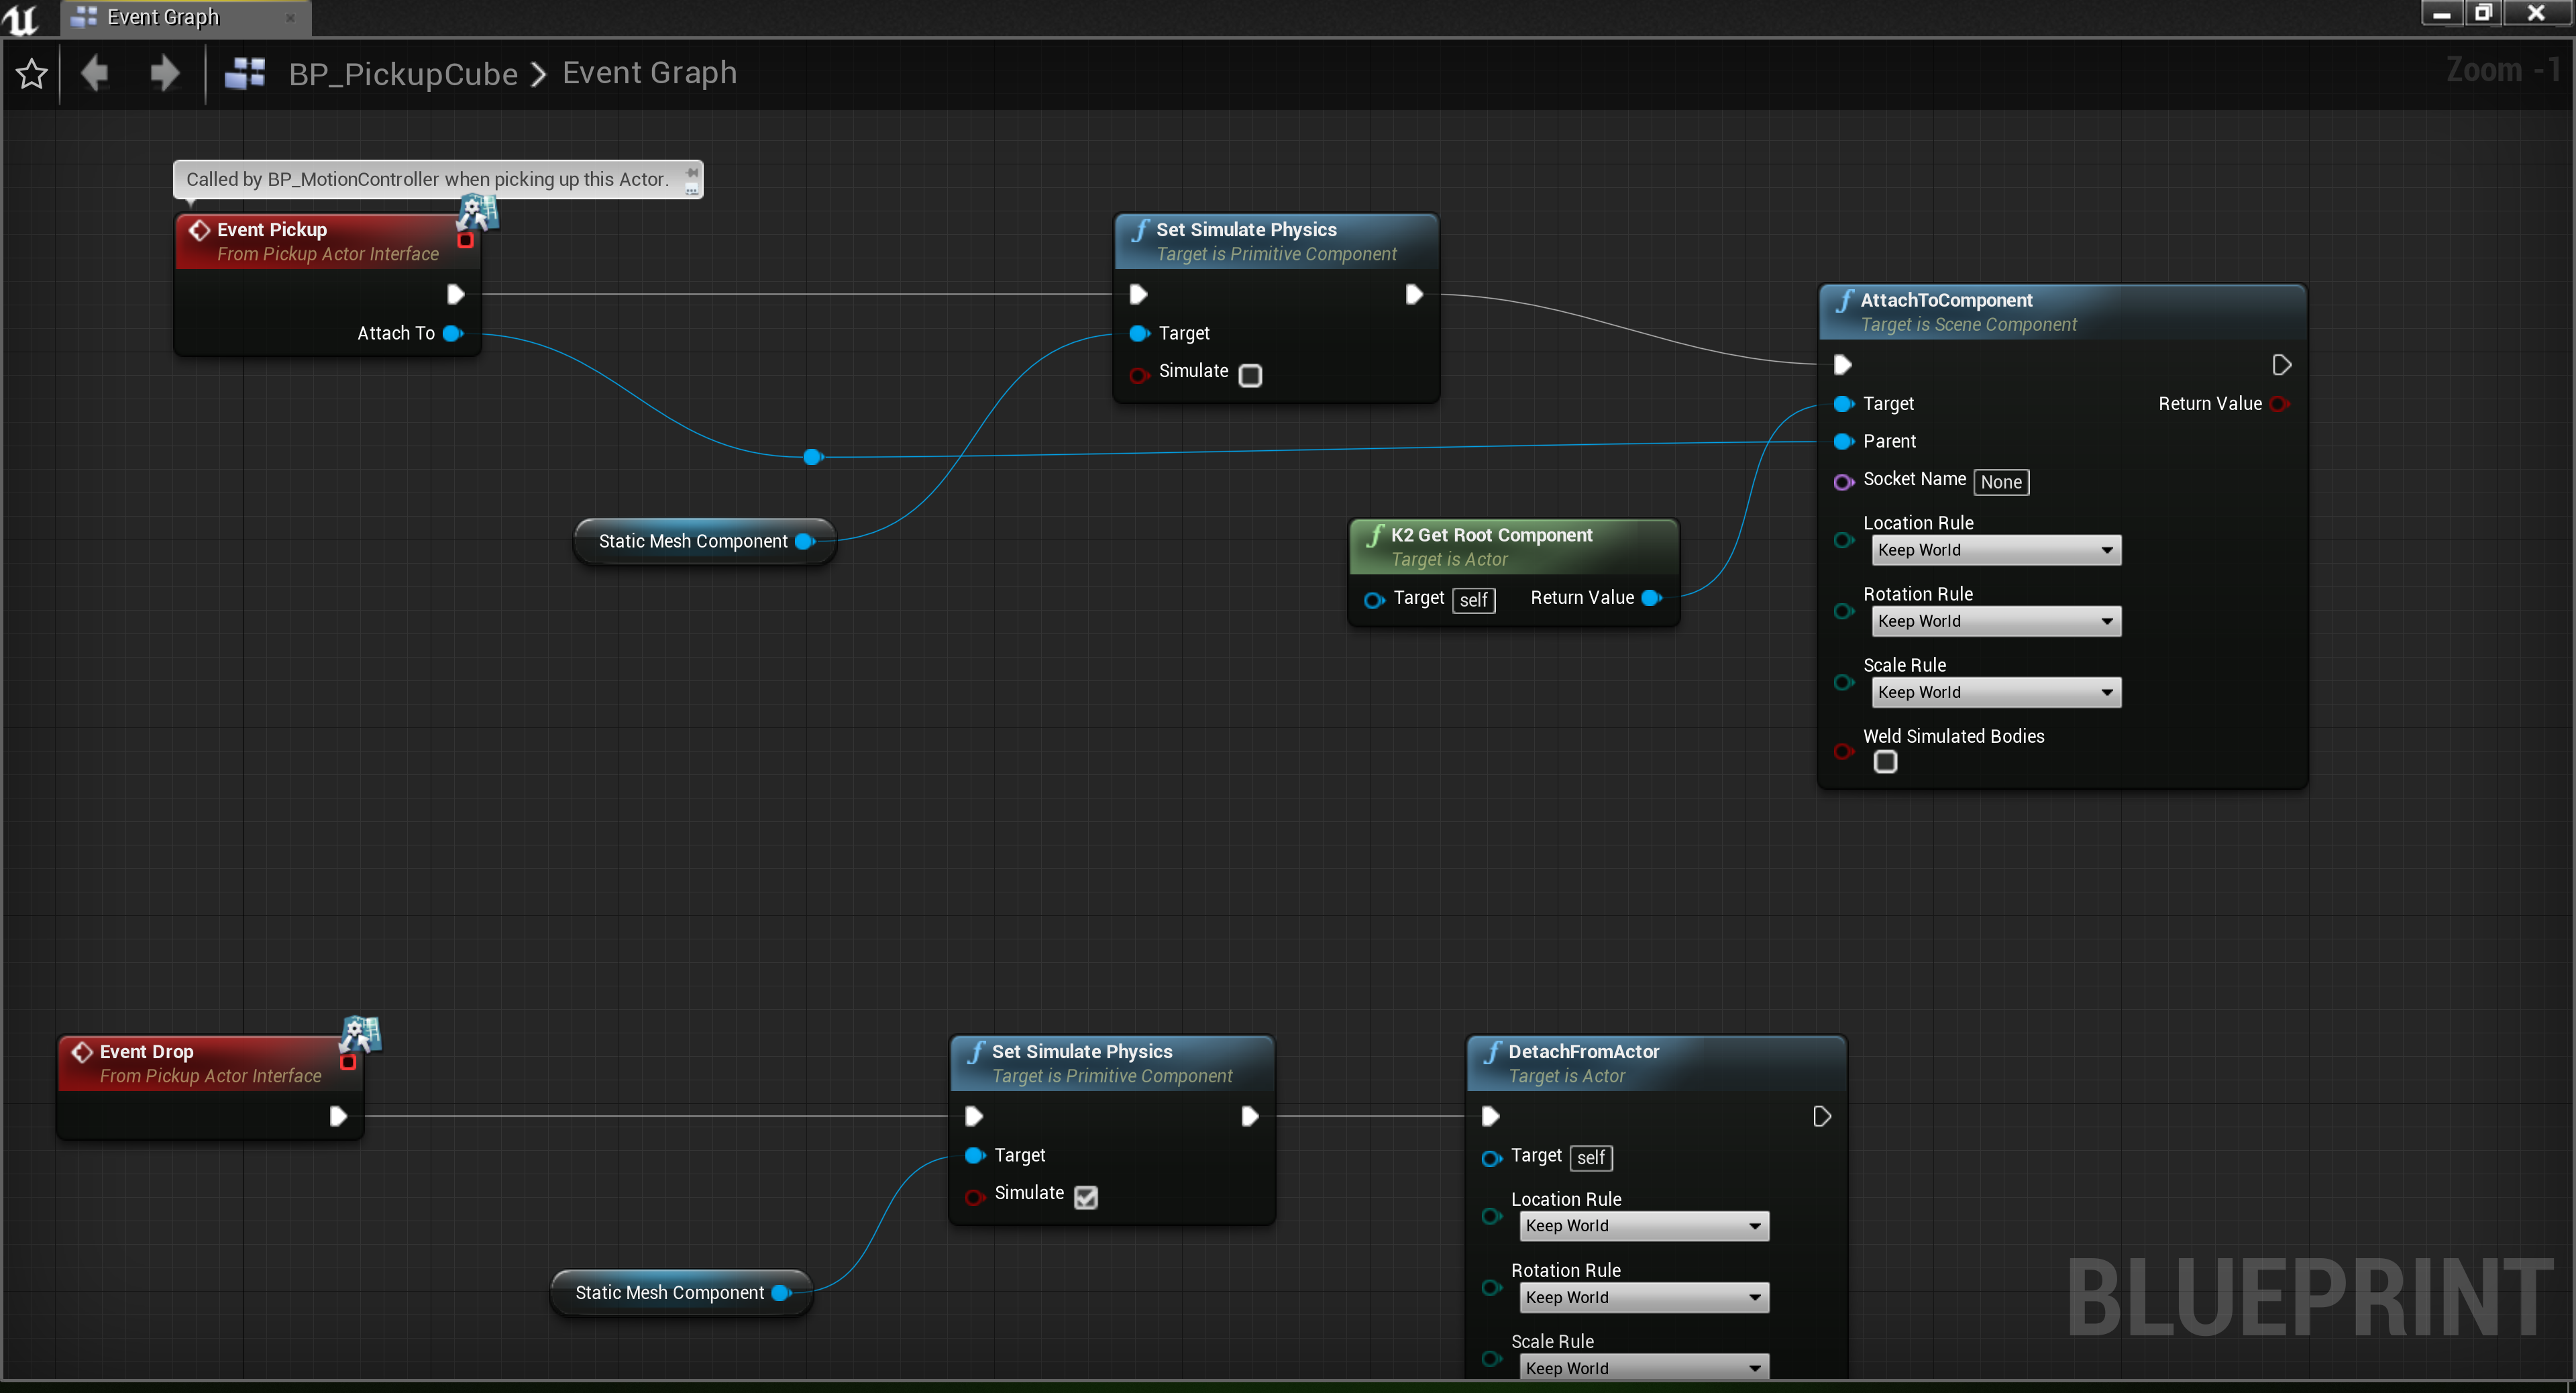
\includegraphics[width=\textwidth]{ue-blueprint-tool}
	\caption{UE4 Blueprint Visual Editor}
	\label{fig:ue-blueprint-tool}
\end{figure}
\par
Blueprints are defined as object-oriented(OO) classes or objects in the engine which is a well known and used programming paradigm. Internally Blueprints are translated to C++ by a VM which comes with a performance penalty \citeyeartitlexamkinline{ue-nativizing-blueprints}. An alternative to Blueprints is using C++ to define the game logic, however in this project Blueprints are favored due to their ability to visually display logic better than code. There are also more examples and snippets online available for blueprints.
\par
Two common types of Blueprints are Level Blueprints and Blueprint Classes. Every level has a Level Blueprint which can manage things like level streaming, objective tracking(checkpoints), interacting with other blueprints in the level. Blueprint Classes on the other hand are used to create interactive assets such as doors, buttons, levers, destructible objects. Main benefit of these blueprints is their reusability. They can be placed in any level and their behavior will remain the same. Also modifying the base blueprint will update all instances of it in the level.
\section{Physics simulation} \label{physics-sim-section}
Unreal Engine provides physics simulation to make experiences more realistic and believable. The physics simulation is done through NVIDIA's PhysX 3.3 physics simulation engine. The main physics simulation tools used in this project are Collision simulations and Traces with Raycasts.
\begin{figure}[H]
	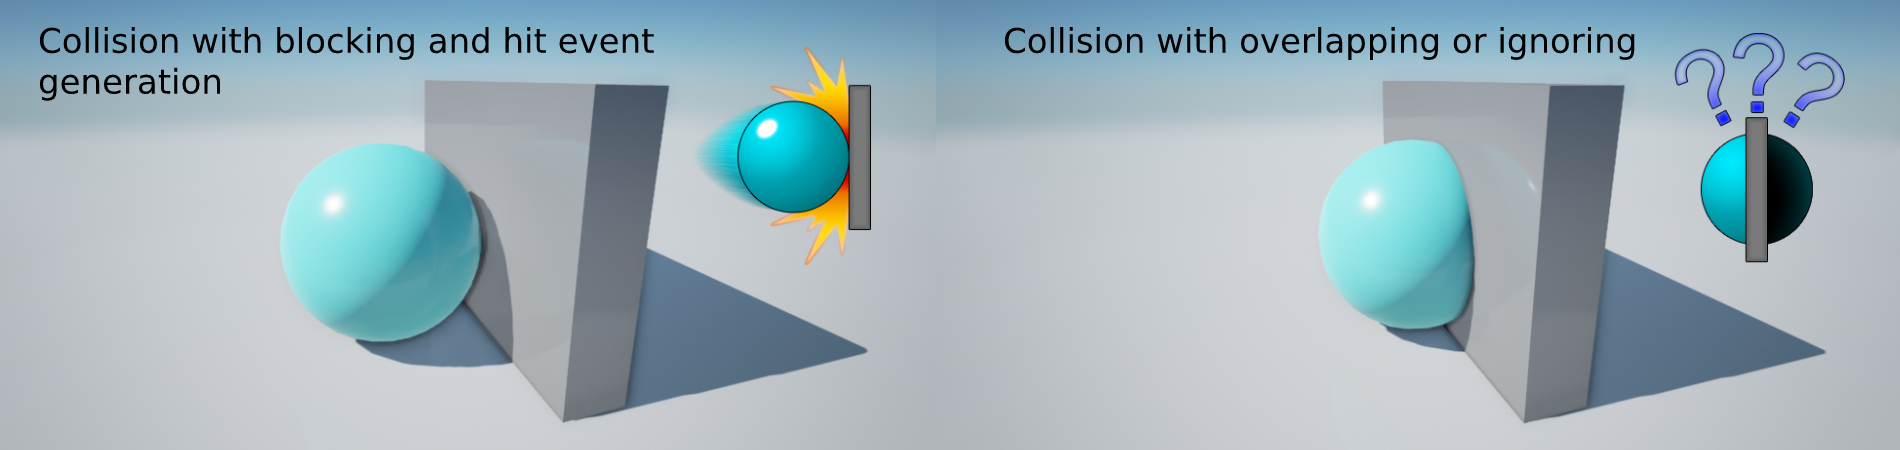
\includegraphics[width=\textwidth]{collision-types}
	\caption{Collision types in Unreal Engine}
	\label{fig:collision-types}
\end{figure}
Objects in the scene have physics and collision settings. These settings are enabled for individual objects rather than for the scene as a whole. The three possible collision response settings are blocking, overlapping or ignoring \Cref{fig:collision-types}. When blocking is enabled on two colliding actors a hit event will be generated. The two actors are unable to overlap eachother and will simply bounce away from eachother. If both colliding actors in stead use overlapping they will go through eachother. If overlap events are enabled for both, overlap events will be generated when the collision begins and ends. If colliding actors use ignore collision they will go through eachother and generate no events.
\par
Traces are straight rays that detect any interescted objects between two points. Intersection of objects generates a trace hit event which supplies a list of the intersected objects. Traces can be ran by channel in which case only objects that are responding to the same channel will be a part of the trace hit event. Additionally single hit and multi hit events can be generated depending on how many times the same object is intersected by the ray. The Trace ray can have a shape of a line, box or sphere. \citeyeartitlexamk{ue-traces}
\section{Static and Skeletal Meshes}
A Static Mesh is a geometry made up of polygons that is cached in video memory and rendered by the graphics card. Being cached in the video memory means that these geometries can be complex and also translated, scaled and rotated in real time. Static Meshes are usually 3D models created in external modelling software and imported to an UE4 project. But primitive meshes such as boxes, cylinders, spheres can also be made in UE4. Objects in the scene such as doors, sensors, batteries, lamps are examples of Static Meshes. \citeyeartitlexamk{ue-static-meshes}
\par
Skeletal Meshes are identical to Static Meshes with the addition of a hierarchical set of interconnected bones, that can be used to animate the meshes' vertices. The Static Meshes, rigging and animations are typically created in external tools like 3DSMax, Maya, Blender \citeyeartitlexamkinline{ue-skeletal-meshes}. These types of meshes are used to create animated objects. In this project the Hi5 VR Gloves are displayed virtually with the use of Skeletal Meshes and animations. VIVE Controllers visualization is also achieved by animating Skeletal Meshes of hands.
\par
Materials define what type the surface of a mesh appears to be. It can be seen as a "paint" applied to a mesh. Materials can define the colour, shininess, roughness, opacity, light emissiveness and many other surface properties. In technical terms a Material calculates how light interacts with a surface. Materials are constructed with a visual scripting tool named Material Editor that is similar to the Blueprint Editor. \citeyeartitlexamk{ue-materials}
\section{Widget Components}
Unreal Motion Graphics UI Designer(UMG) as a visual editing tool used to create 2D interfaces for the Unreal Engine. This is often used to create widgets such as HUDs(Head-up displays), menus, 2D animations, user input fields. Some examples of UMG elements are checkboxes, text, buttons, progress bars, 2D images, sliders. The designer has two main views. Designer view which allows the user to edit widgets and also see how they  will look in the application. And a Graph view which is used to assign logic and functionality to the widgets.
\par
Widgets created with UMG can be added to a scene in two different ways. The first method is to create a new widget instance of the widget and add it to the Viewport. In this case the widget will be truly 2D as it will be always facing the camera at the same angle and from the same position. This approach is useful for creating UI interfaces that need to be constantly present on the screen, like game score, healthbars or time counters. The second method for introducing UMG Widgets to the scene is by using a Widget Component. The Widget Component overlays the 2D UMG Widget on a 3D plane. The Widget Component has 3D world transform, meaning it has a set position and orientation in the scene. The 2D interface is projected on the surface of the Widget Component plane similarly to a Material. However this approach is more suitable for creating assets of TV's, pictures, signs than using Materials, due to the simpler management of Widgets for 2D interfaces. \citeyeartitlexamk{ue-umg}
\par
\chapter{\texorpdfstring{Project implementation}{proj-impl}}
This chapter covers the practical implementation of the project application. Level layout and design is created and explained. Blueprints defining the game logic are also created and explained. Other various steps of the implementation process are listed and discussed.
\section{Project setup}
The project application will be developed in the Unreal Studio software. Unreal Studio comes with a new Project wizard and several templates for new projects. The template most suitable to this project is the Virtual reality Blueprint template. It comes with optimized graphics settings for VR and example blueprints for common VR operations \Cref{fig:new-project}.
\begin{figure}[H]
	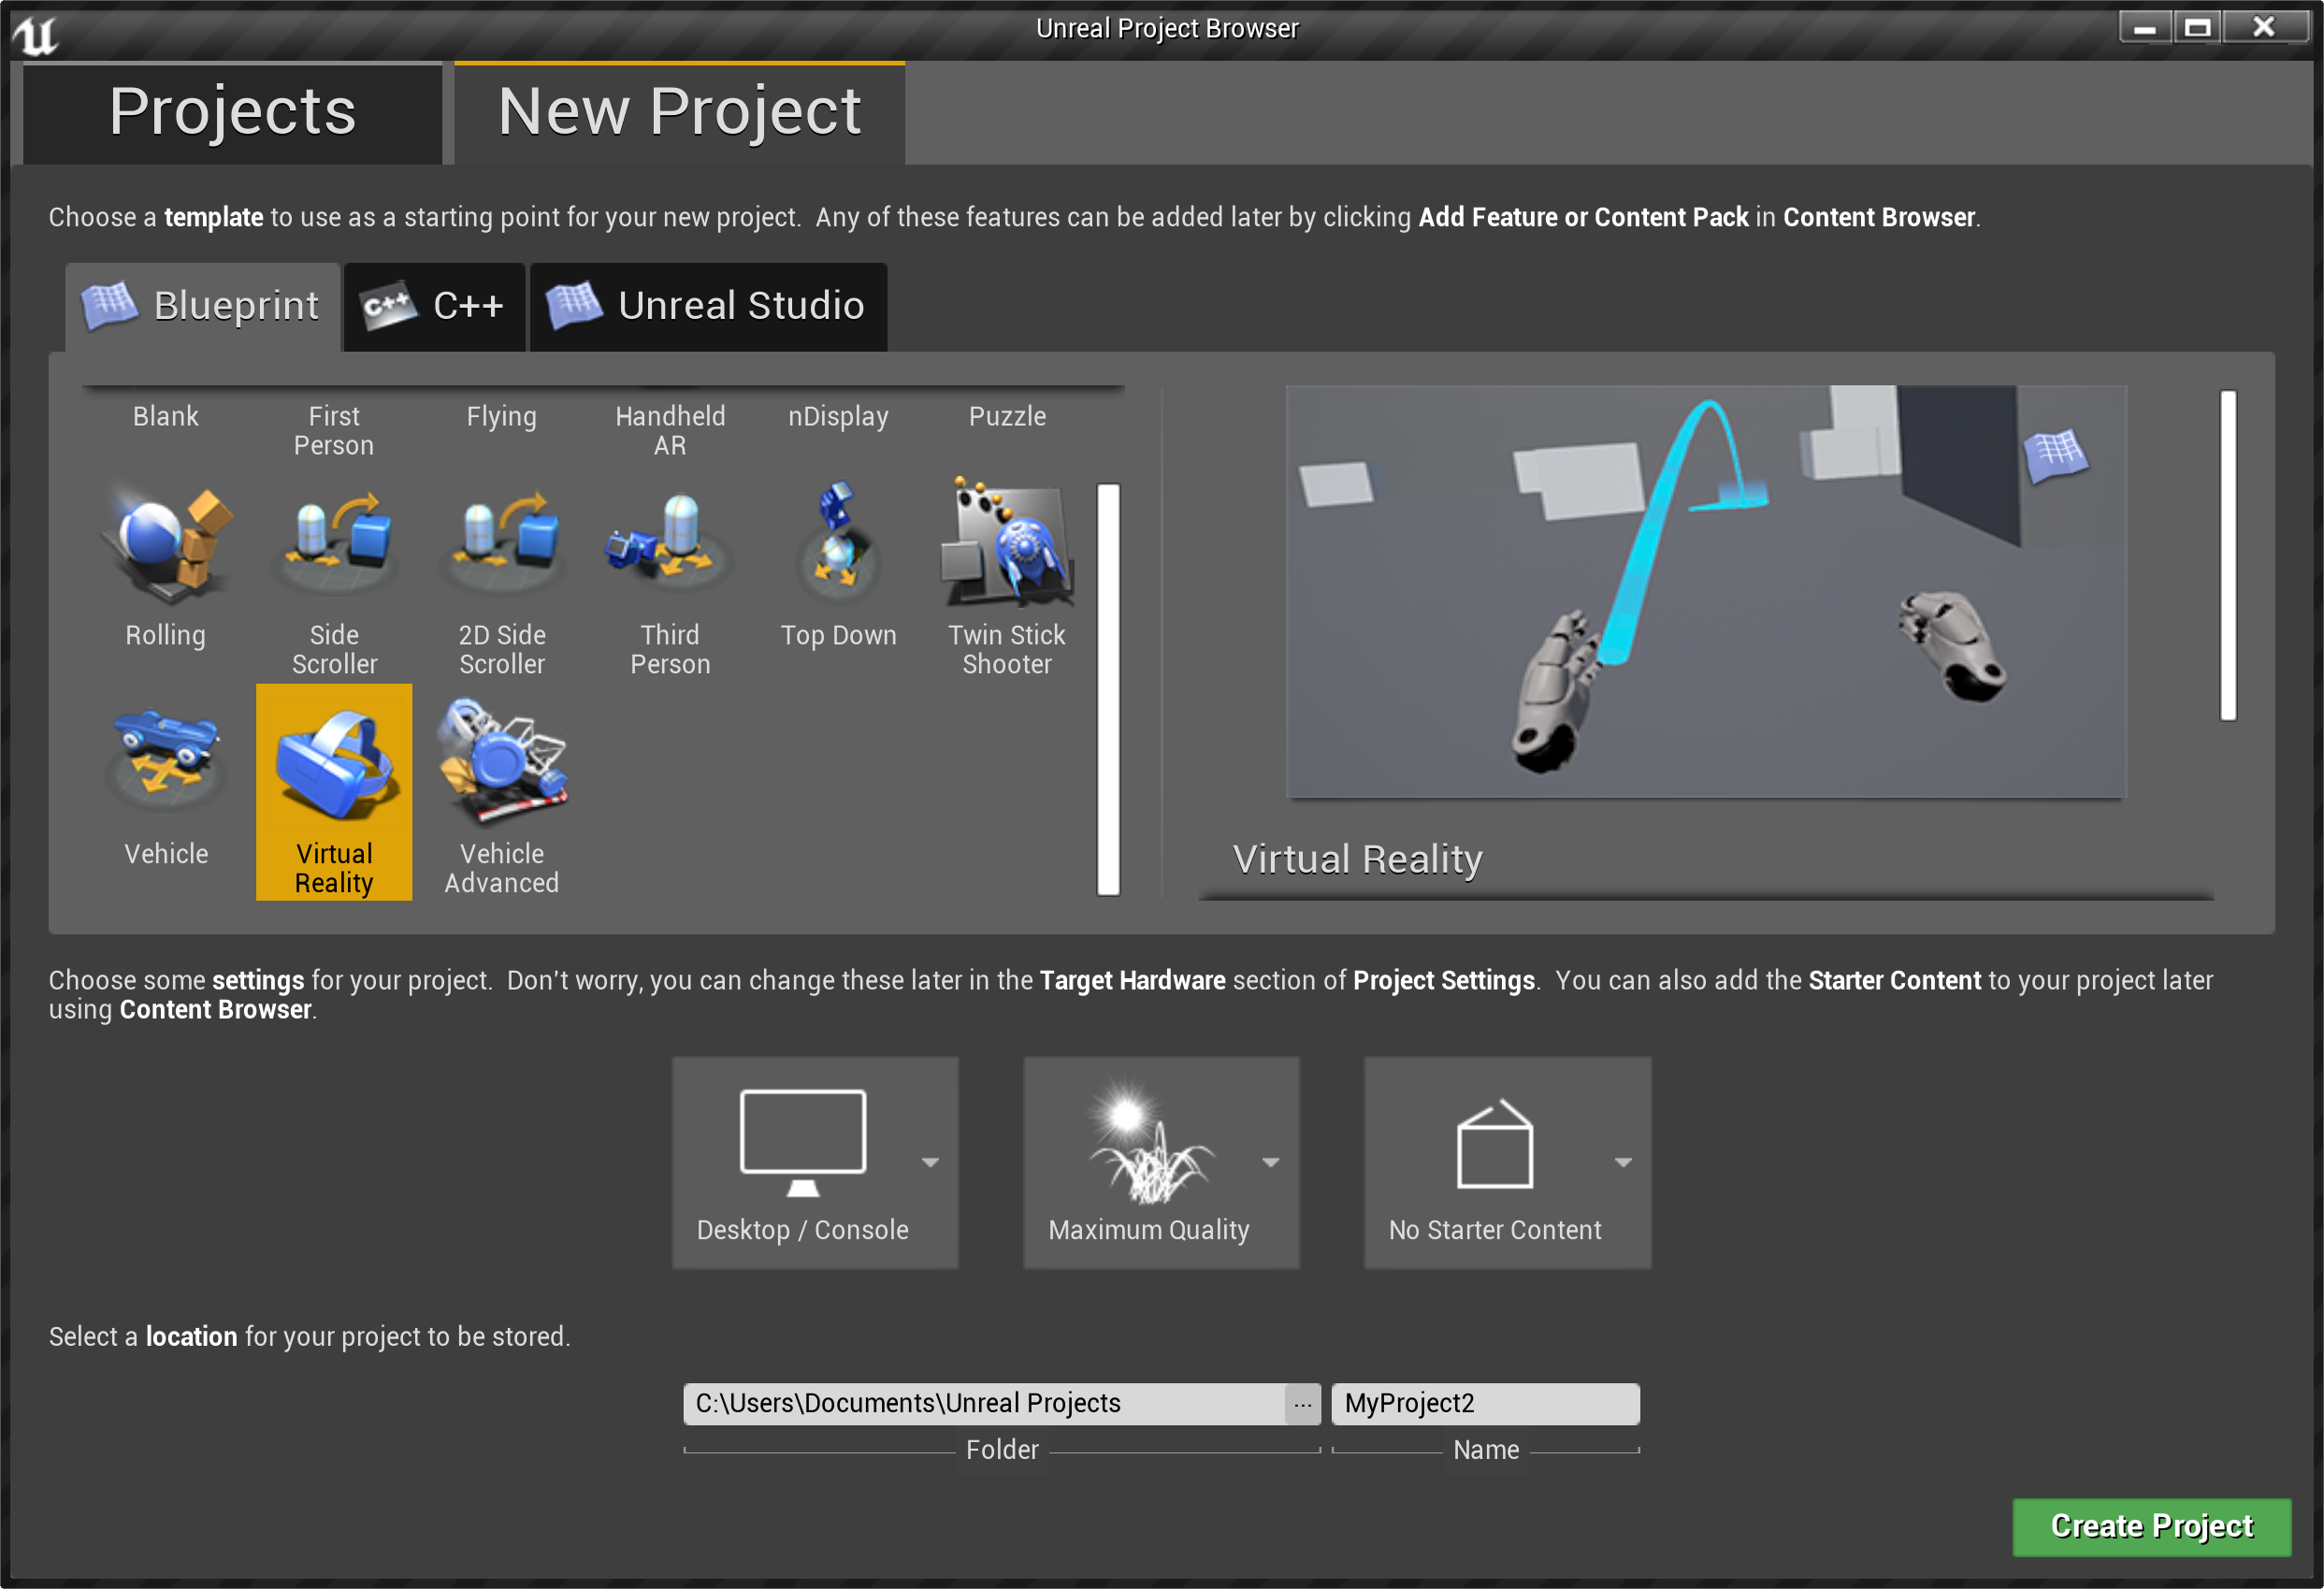
\includegraphics[height=250pt]{new-project}
	\caption{Unreal Studio new project wizard}
	\label{fig:new-project}
\end{figure}
General project preferences can be selected for the project during the creation process. Target platform for the application and rendering quality options are available. These options pre-configure the project to best suite the needs of the application. Changes can be made to the project settings later on if needed. It is possible to add starter content to the project which includes several levels, static meshes and blueprints and can be ran straight away as a VR demo application.
\section{Level design}
Level design begins with the layout and orientation of the different meshes. The visual appearance of the level is made more realistic by using different textures, materials and lighting. A vehicle 3D model is used as the center point for the level and also for the player starting point.
\par
The player starting point is placed in the interior of a conversion van \Cref{fig:vehicle-interior}. If the starting point Actor is colliding with objects in the scene an icon "BADsize" will appear. This means that the starting point is invalid and the engine will try to find the nearest valid starting point. During the development process the camera location in the editor can be used as a strating point which speeds up testing. \citeyeartitlexamk{ue-playerstart}
\begin{figure}[H]
	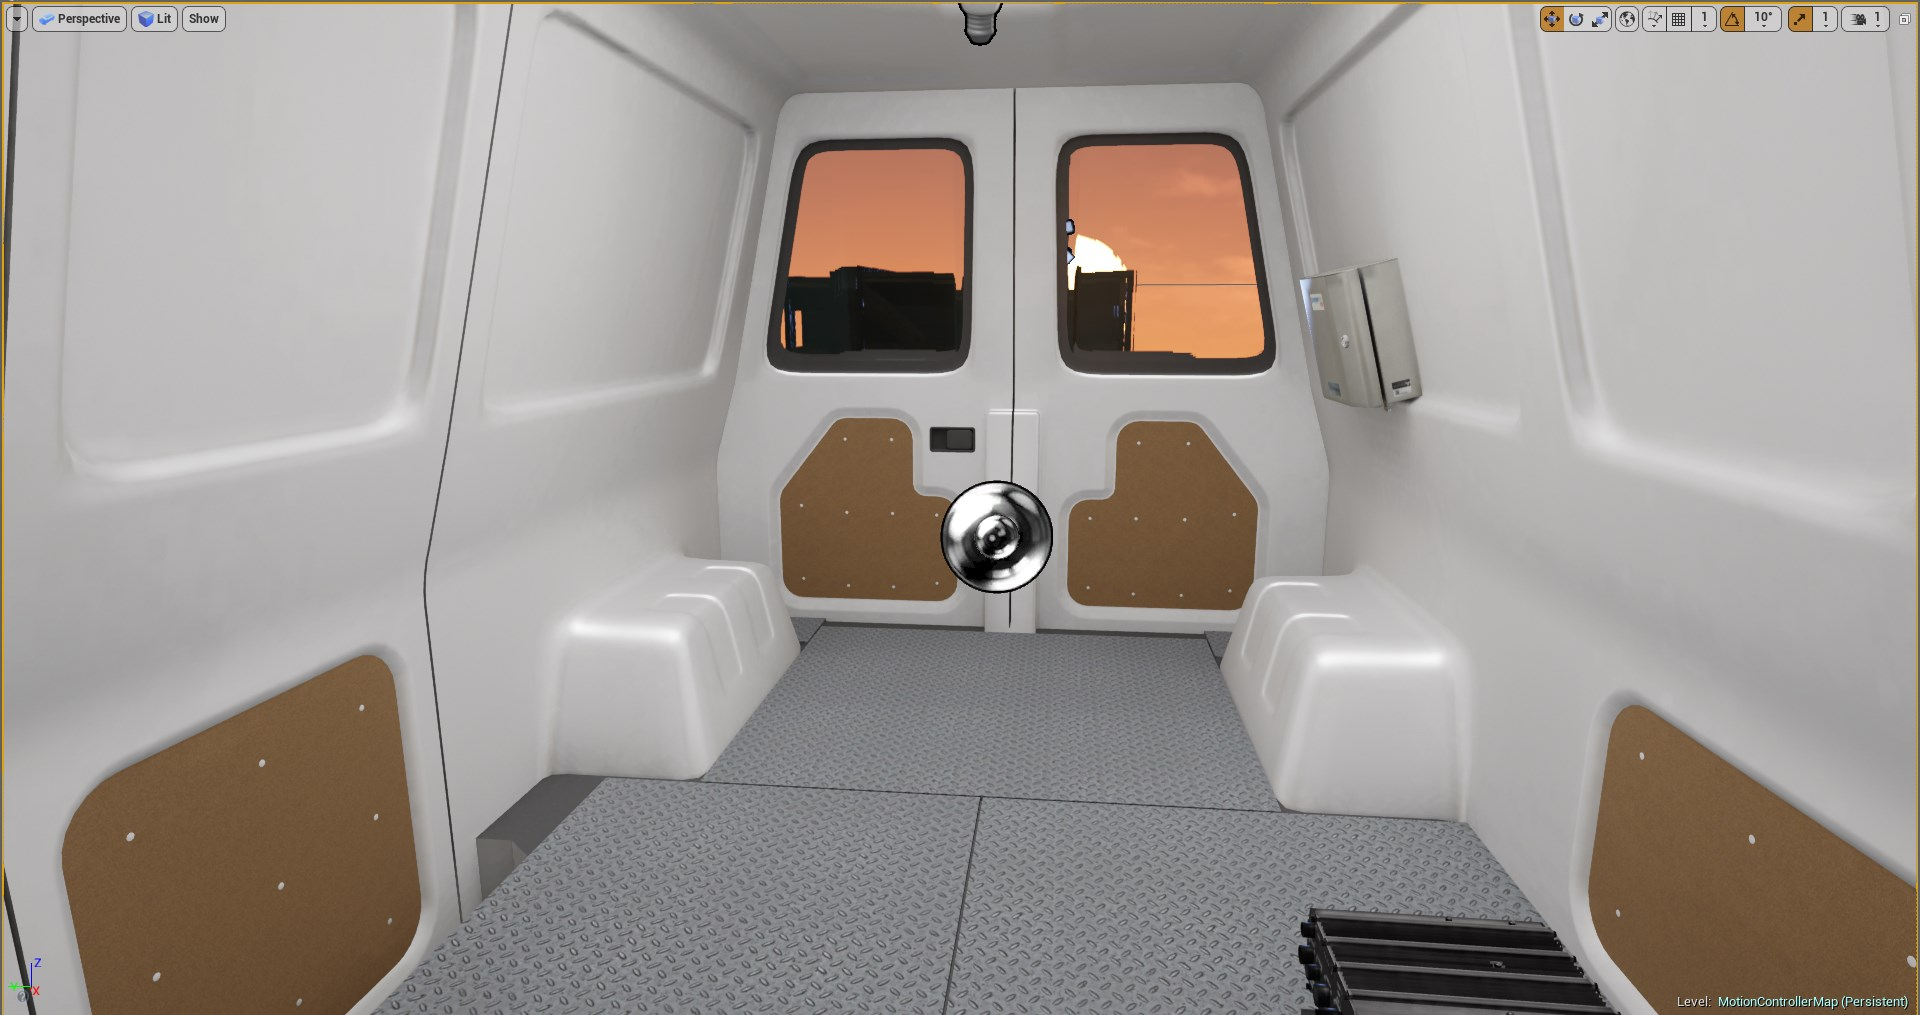
\includegraphics[width=\textwidth]{vehicle-interior}
	\caption{Starting Level Vehicle Interior}
	\label{fig:vehicle-interior}
\end{figure}
\par
Light sources are required to make meshes in the scene visible to the user. Two primary light sources are used in this level. The first light source is a Directional Light and is used to simulate the sun. Directional lights simulate a light source that is infinitely far away which means all the shadows cast by the light are parallel. This makes Directional lights perfect for simulating sunlight. This light is also Moveable which means its location and orientation can change on runtime. This can be used to cast dynamic shadows, but in this project dynamic shadows will be disabled to improve the rendering performance. The second light source is located inside the vehicle and is used for interior lighting. The type of this light is Point Light. Point Lights are used to simulate light bulbs because they emit light in all directions. \citeyeartitlexamk{ue-lightsources}
\par
A SkySphere(Skydome) is used to create a background for the scene that simulates a sky. While the player is moving in the scene the SkySphere remains stationary which gives the illusion that the sky is very far away. A 2D texture is wrapped on the inside of a sphere to create a SkySphere. The SkySphere in this project is also dynamic. Clouds are moving and the Directional Light source mention in the previous paragraph is moved by the SkySphere to simulate day and night cycles. The intensity and color of the light source is also changed depending on the time of the day.
\section{Glove calibration and tracking}
Hi5 VR Gloves require the user to go through a calibration process before use to ensure better finger tracking. This process needs to be done if the gloves have been turned on or a new person is going to be using the gloves. Noitom, the creators of the gloves, provide a sample UE4 project that includes the calibration process with instructions for the gloves. The calibration can be done with the stand-alone sample project, but to keep the final project self-contained the calibration will be added to the application.
\begin{figure}[H]
	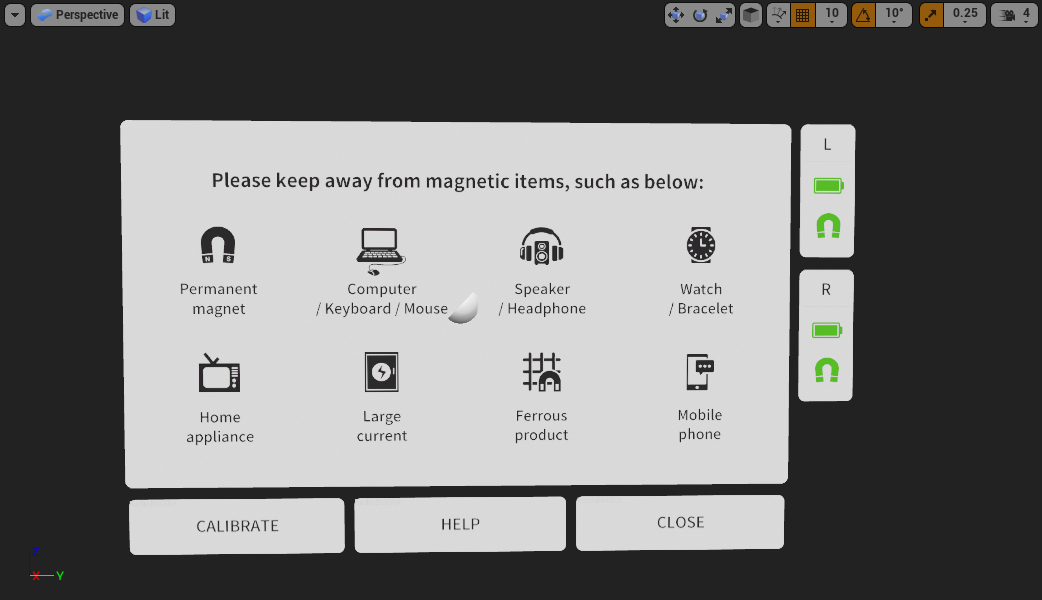
\includegraphics[width=\textwidth]{calibration-menu}
	\caption{Glove calibration menu and instructions}
	\label{fig:calibration-menu}
\end{figure}
\par
Inspecting the assets of the sample project reveals that several actors are responsible for the instructions and calibration of the gloves. The UE4 editor comes with an asset migration tool which is used in this case to migrate these actors to the ObSAS VR project. The MainLogicActor contains instructions and menu with options to calibrate the gloves. It uses WidgetComponent children for the instructions and selection buttons \Cref{fig:calibration-menu}. Glove battery and magnetisation status are also shown. The InteractionPawn Blueprint Class is mainly responsible for the camera projection. The camera view is bound to the tracked real world location of the VR headset. This means that if the user moves or rotates in the real world the camera view will update its orientation and position and render different parts of the scene. A WidgetInteractionComponent is a part of this Class. This component contains a Static Mesh in the shape of a small square. This mesh is used as a pointer for the user, it is located in the center of the camera projection at all time. If the user positions the camera in such a way that this pointer overlaps a menu option a countdown timer will start. If the pointer is not moved outside of the menu option the countdown will end and the option will be selected \Cref{fig:calibration-menu}.
\begin{figure}[H]
	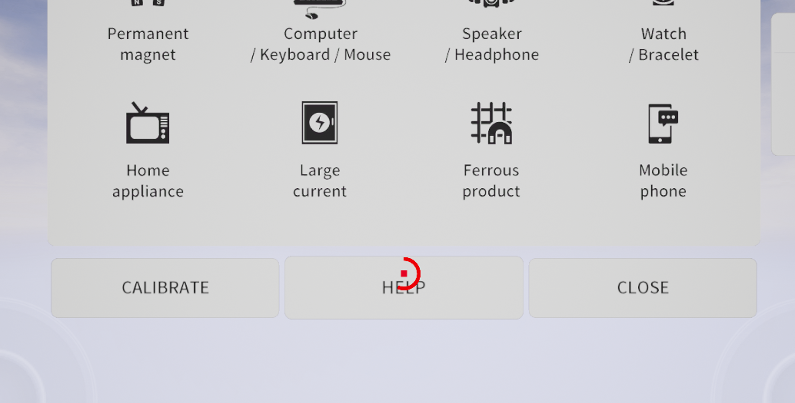
\includegraphics[width=\textwidth]{menu-selection}
	\caption{Camera pointer and menu selection}
	\label{fig:menu-selection}
\end{figure}
The calibration process requires the user to perform two hand gestures for a period of time. Calibration data is used and created by the Mocap plugin. GameInstance Blueprint Class is responsible for starting and stopping the Motion Capture service from the Mocap Plugin. This UE4 plugin is provided by the glove manifacturers. It provides relative tracking of the integrated sensors on the gloves. Combining this relative data with the absolute positioning data from the VIVE Trackers full hand and finger tracking is achieved in VR.
\section{Interacting with the virtual environment}
Interacting with the virtual environment is possible in three different ways. Firstly using the camera pointer method described in the previous chapter. Secondly by using the Hi5 VR Glove. Lastly the VIVE controllers can be used to grab objects.
\par
VIVE controller interaction method is required as a backup to the Hi5 VR Gloves. Magnetic interference or radio frequency interference can make the gloves' tracking inaccurate, unreliable or even completely prevent it. This is not a huge problem during training as the environment can be controlled and time is not limited. Furthermore interference can be removed and the gloves can be demagnetized and recalibrated. However if the application is used in public exhibitions interference can be a real problem.
\subsection{Gloves interaction}
Using gloves to interact with objects in the virtual environment can be achieved with simulated physics. The gloves are tracked and represented in the scene with a Hands Actor. The hands meshes in the Hands Actor are configured with a collision preset of Block All Dynamic. As explained in section \ref{physics-sim-section} this means that other meshes with the same collision preset will not be able to go through(overlap) the hands meshes. In stead a hit event will be generated when a collision occurs and the colliding actors will be pushed away with a force. The force depends on the velocity, mass and force modifier property of the colliding meshes.
\begin{figure}[H]
	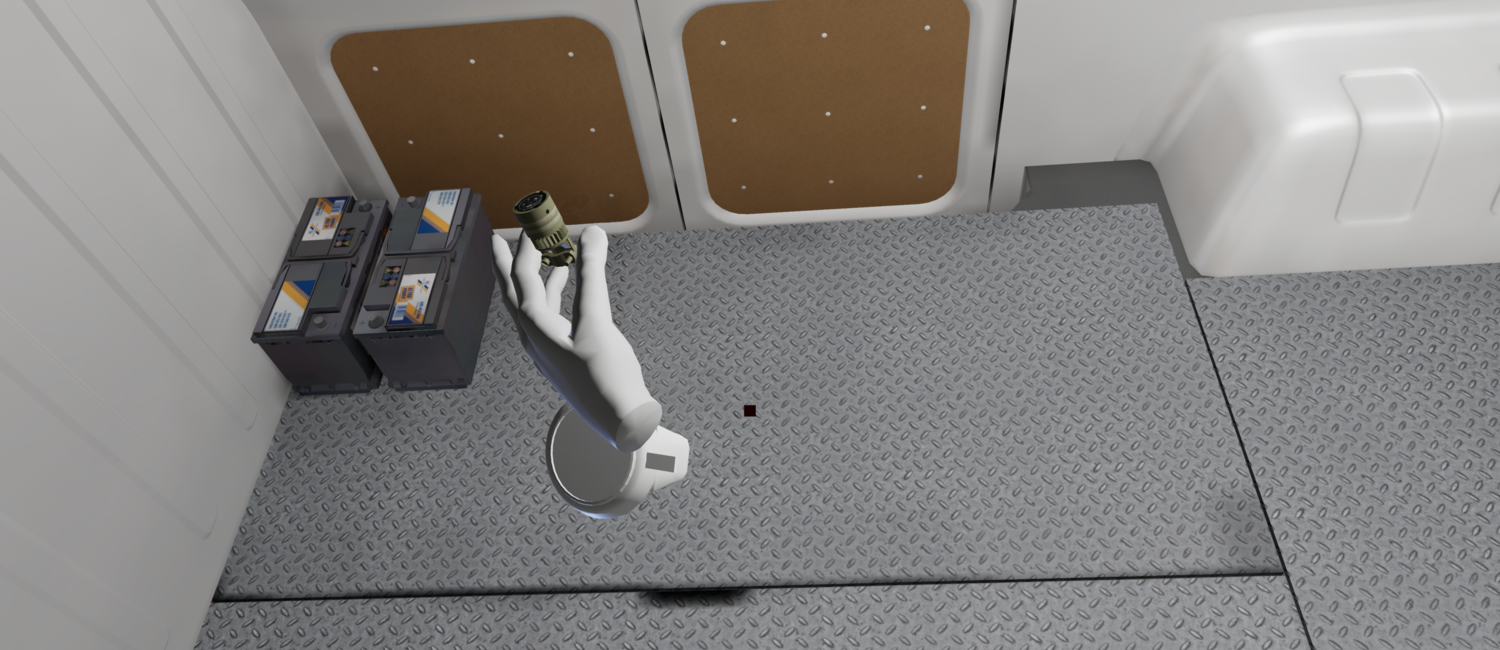
\includegraphics[width=\textwidth]{gloves-grab}
	\caption{Holding object with gloves}
	\label{fig:gloves-grab}
\end{figure}
Holding and moving objects becomes possible with these settings. The interaction is similar to real life hand interaction \Cref{fig:gloves-grab}. Hands and objects block eachother on the surface level and do not overlap. One main difference is the haptic feedback real life interaction provides. A person feels the surface of objects, but in VR it is only feasible to have visual feedback. Hi5 VR Gloves have vibration feedback, but this is not isolated to individual fingers, it rather affects the whole glove. This makes vibration feedback unusable for feeling surfaces.
\par
 Collision simulation is computationally expensive and also not deterministic. Objects with locked position such as buttons and levers can behave strangly when using collision physics \citeyearxamk{collaborative-vr}. Because of these reasons a more suitable approach is used to simulate these kind of object interactions. For buttons interaction a trace box surrounding the button is created. This trace box has no visual representation, so it cannot be seen by the user in the scene. The trace box uses overlapping collision and allows other meshes to pass through it, generating overlap events. When a hand mesh overlaps the trace box an overlap event with a distance parameter is generated. This parameter indicates how far the hand has entered into the trace box and is used to determine if a button is pressed. Rotary switches and levers use a similar approach but rather than using a distance parameter they use the hand mesh location and rotation.
\subsection{VIVE Controllers interaction}
HTC VIVE Pro comes with a pair of wireless motion controllers. These controllers are tracked by the base station of VIVE and their primary use is for interaction with the VR world. The controllers have several buttons and a trackpad which provide more interfacing capabilities \Cref{fig:motion-controller}. Motion Controllers will be used as a backup to Hi5 VR Gloves during exhibitions and also during the development process thanks to the quicker setup for usage.
\begin{figure}[H]
	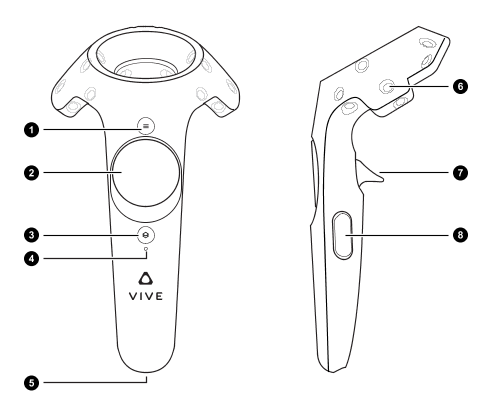
\includegraphics[height=230pt]{motion-controller}
	\caption{HTC VIVE Pro Motion Controllers}
	\label{fig:motion-controller}
\end{figure}
Unreal Engine provides a Motion Controller(MC) Component that offers support for commonly used VR MC brands. VIVE Motion Controllers are supported by this Component. Two instances of this Component are added to the Camera actor, as the location of the controllers is relative to the Camera location which itself is locked to the location of the VR headset. A static mesh of a mannequin hand is added as a child to each MC Component. One is for the right hand and the other for the left hand. Since only a mesh of the right hand is available this mesh needs to be mirrored in the Y-coordinate for the left hand. After these steps the hand meshes should be visible in the scene and their position follows the controllers' position.
\begin{figure}[H]
	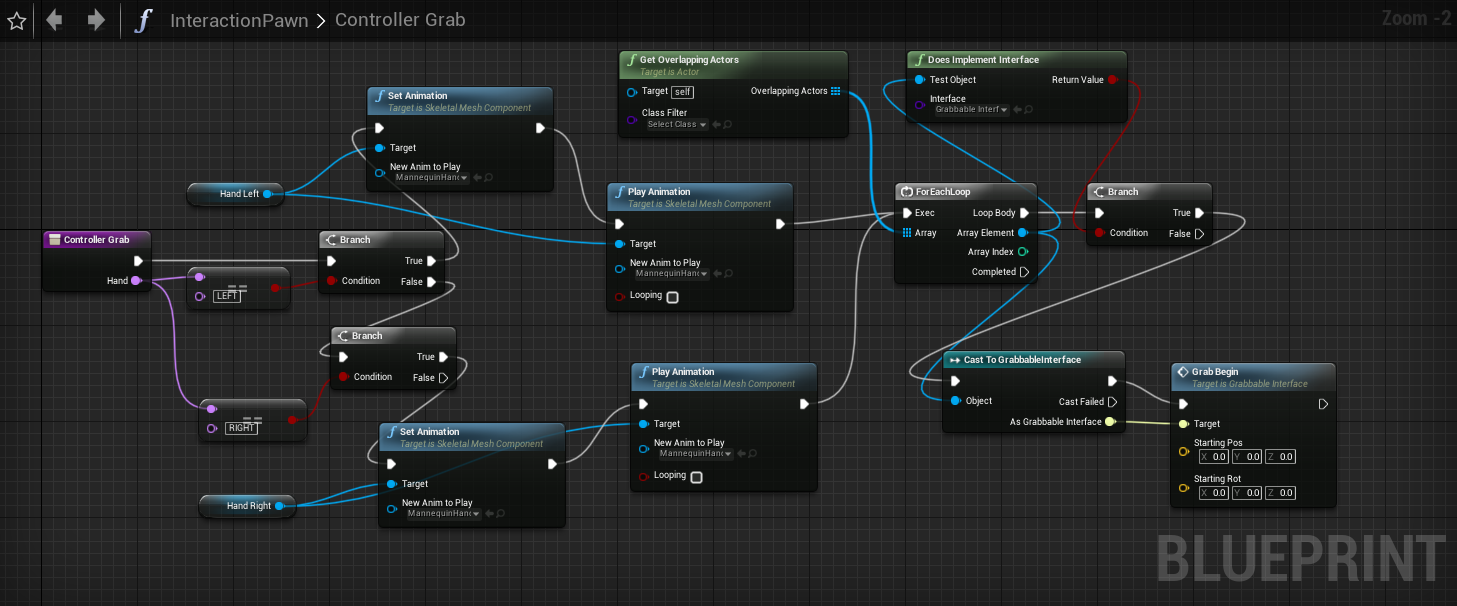
\includegraphics[width=\textwidth]{grab-blueprint}
	\caption{Logic for Motion Controller grabbing}
	\label{fig:grab-blueprint}
\end{figure}
Interacting with other objects in the scene is done by utilizing overlap events while pressing the Motion Controller trigger button \Cref{fig:motion-controller}. The trigger button press and release events are available in the Blueprint Editor. They're used to create grab and release functions that fire grab and release events on objects that are overlapping with MC meshes. The hands' mesh is animated when the trigger button is pressed. It changes from an open palm hand to closed palm hand, visualizing that grabbing has been initiated. An interface for objects that can be grabbed is created and implemented by every object that needs grabbing functionality. The overlapped actors are iterated after playing the grab animation and checked for implementation of the Grabbable Interface. Actors implementing the interface then have the GrabBegin function called and decide what grabbing behavior they have \Cref{fig:grab-blueprint}. If the object is something that can be carried its position and rotation will follow the MC until released. If the object is a rotary switch it will follow the MC rotation in one axis. If the object is a lever only movement in one axis will be used.
\section{Virtual hardware layout and operation}
Hardware layout needs to be planned to be both realistic and simplified for VR use. Creating an absolute clone of the real environment at this point is not only unfeasible due to the time constraint, but also distracting for the user as a majority of the hardware is not of importance during the CBRN training. Additionally having 3D models of all the real hardware in the scene can lead to performance penalties that would require more work on optimization or higher-end PC hardware to run.
\subsection{Devices and sensors}
The sensors available at this point of the development are ChemProFXi(chemical detection and classification) and IdentiFINDER S900(radiological detection and identification). In the future IBAC2 will be added to provide biological detection. Weather sensor in the real project is Vaisala WXT536, but a 3D model isn't needed for the current application because the trainee is not able to leave the vehicle. In stead measurement values are simulated with a random number generator.
\par
Additional devices are present in the virtual environment that are crucial to the operation of the ObSAS installation. Two 12V 95Ah batteries are installed in the vehicle as a power source of the system. A power and data distribution box is used to provide fuse protected power from the batteries to all devices. In the case of a device short circuiting the rest of the system will still receive adequate powering. The box also connects data inputs and outputs between the different devices. A laptop computer and a touchscreen are present for interfacing with the ObSAS Software. A lamp provides light to the interior of the vehicle. A military spec computer TRAX-10 is mounted to the wall. This computer records input from all devices and runs the ObSAS software.
\par
Some considerations have been taken for the realisticity of the device layout:
\begin{itemize}
  \item Batteries are close to the power box to avoid creating interference and voltage drop.
  \item Devices are mounted flat to the walls using their mount points.
  \item Batteries are placed on the floor and held with a bracket to avoid unintentional movement.
  \item Air outlets on the ChemProFXi go to the outside of the vehicle. This avoids pushing contaminated air into the vehicle.
  \item All devices have cabling to the power box for data and power.
\end{itemize}
\subsection{Wiring devices}
Devices in the system require DC power to operate. Devices also communicate between eachother via Ethernet or RS232/485 protocols. Powering devices requires power cables and data exchange requires data cables. Two types of cable components can be used in the scene. Dynamic cable actors are used for objects the user can interact with. Static cable actors are used only for visual representation of cables, these actors cannot be modified during runtime.
\begin{figure}[H]
	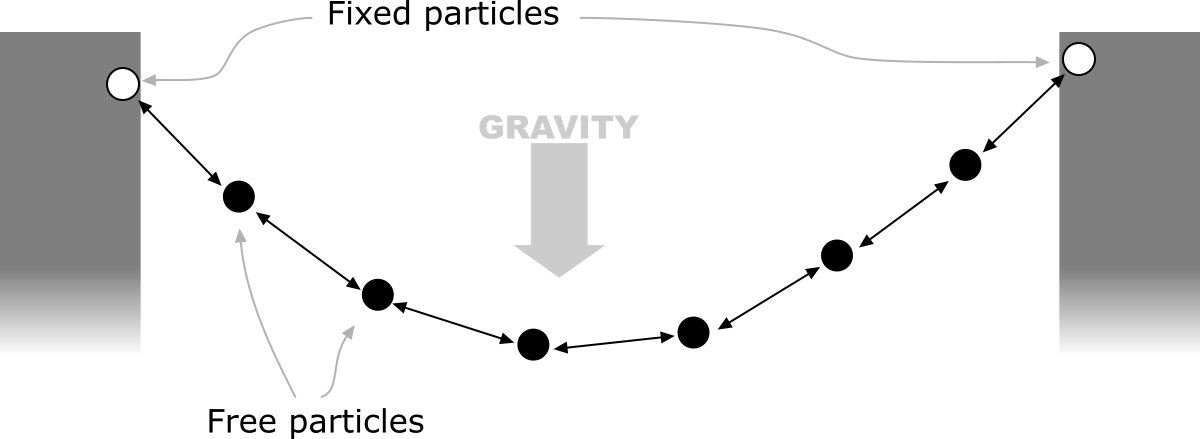
\includegraphics[width=\textwidth]{particle-rope}
	\caption{Cable Component Simulation \citeyeartitlexamkinline{cable-component}}
	\label{fig:particle-rope}
\end{figure}
\par
Dynamic cable components are needed for interactive objects such as connectors with an attached wire. Unreal Engine provides a Cable Component Plugin that is suitable for this use. The Component has start and end attach points with fixed location. Between those points series of free moving particles are located. These points are separated by a distance constraint and use simulated physics to determine their location \Cref{fig:particle-rope}. The cable simulation is done by attaching the start point to a connector and the end point to the distribution box. When the connector is held and moved around the world the cable will follow it with natural movement by bending and bouncing \Cref{fig:cable-grab}. Physics simulation is also used to block cable collision with other actors, without this the cable will go through actors in the scene.
\begin{figure}[H]
	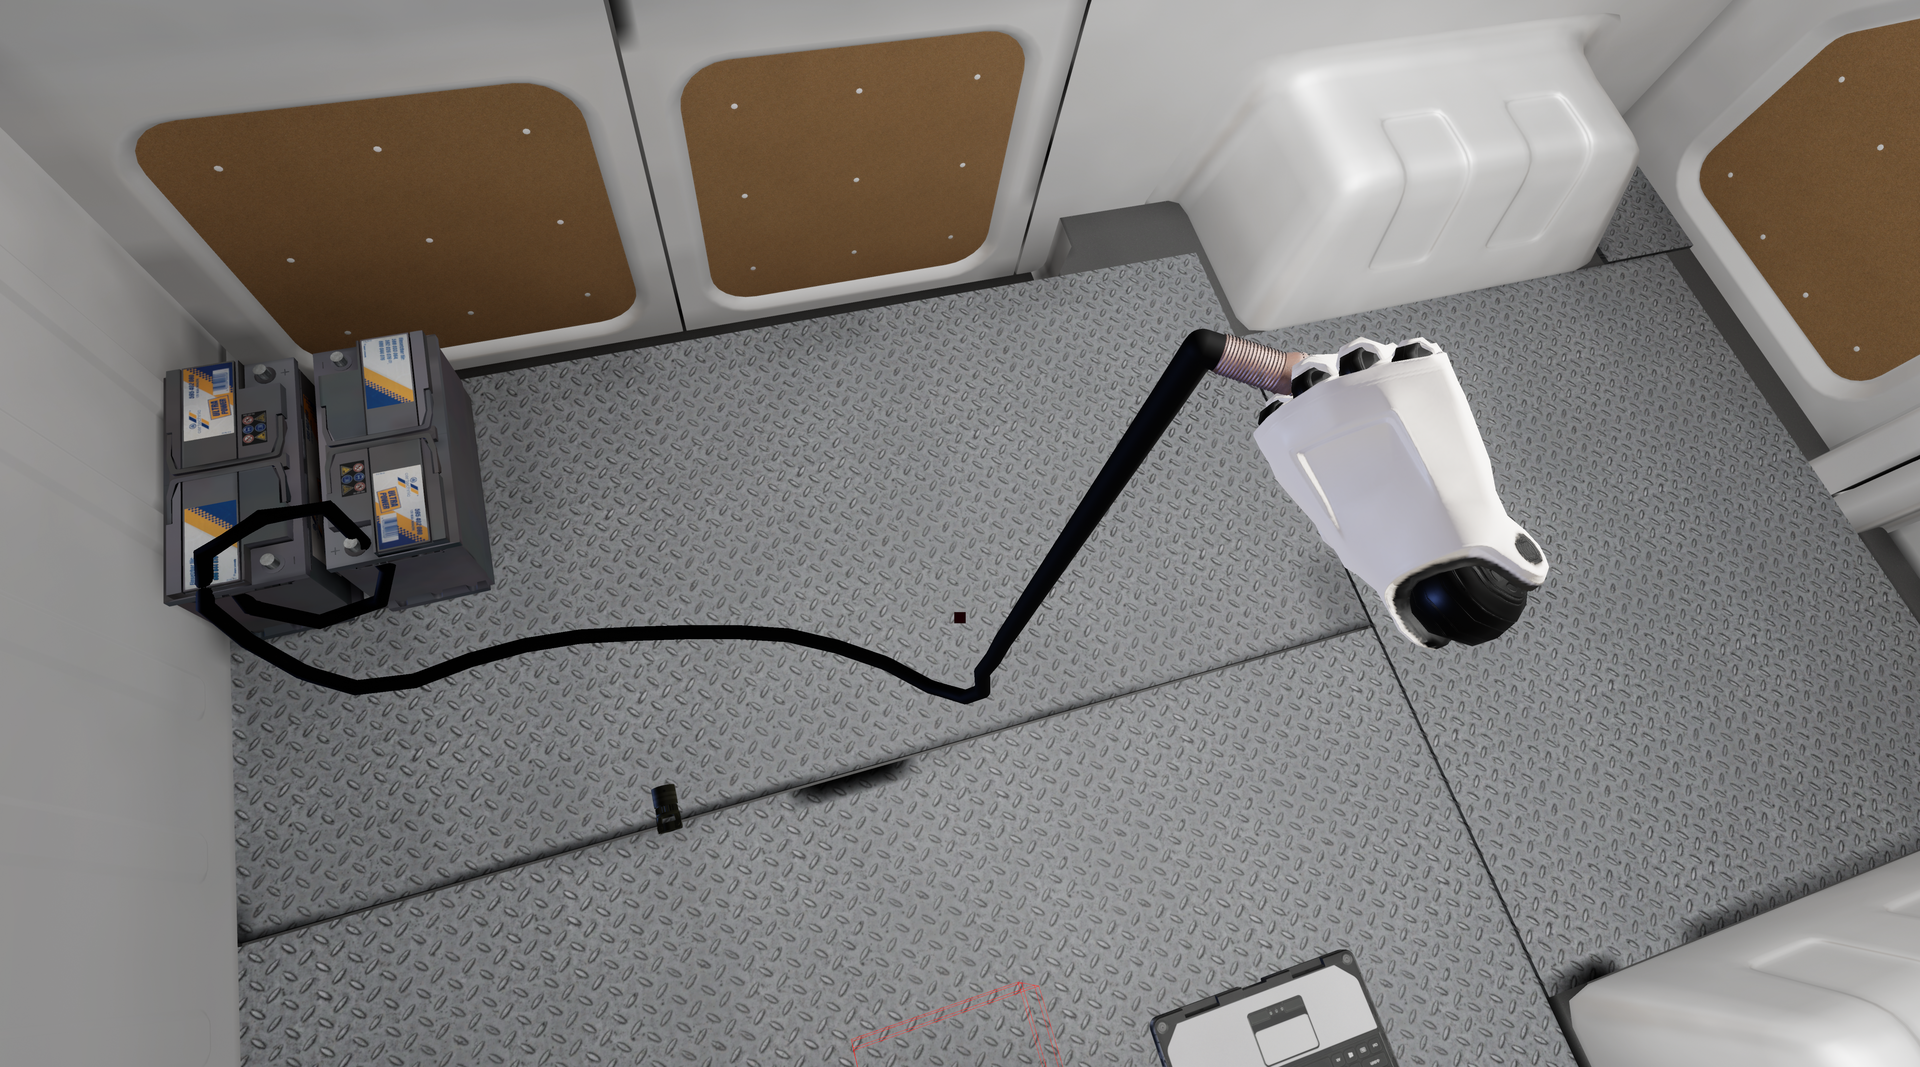
\includegraphics[width=\textwidth]{cable-grab}
	\caption{Cable Component attached to objects}
	\label{fig:cable-grab}
\end{figure}
\par
Static cables in the scene do not move during runtime. These cables are used for connecting objects in the scene that also do not change location. One example for such a cable is the connection between the Power Distribution Box and TRAX-10 computer. Neither of those components are designed to be moved by the end user so the cable between them doesn't need to be movable in VR either.
\begin{figure}[H]
	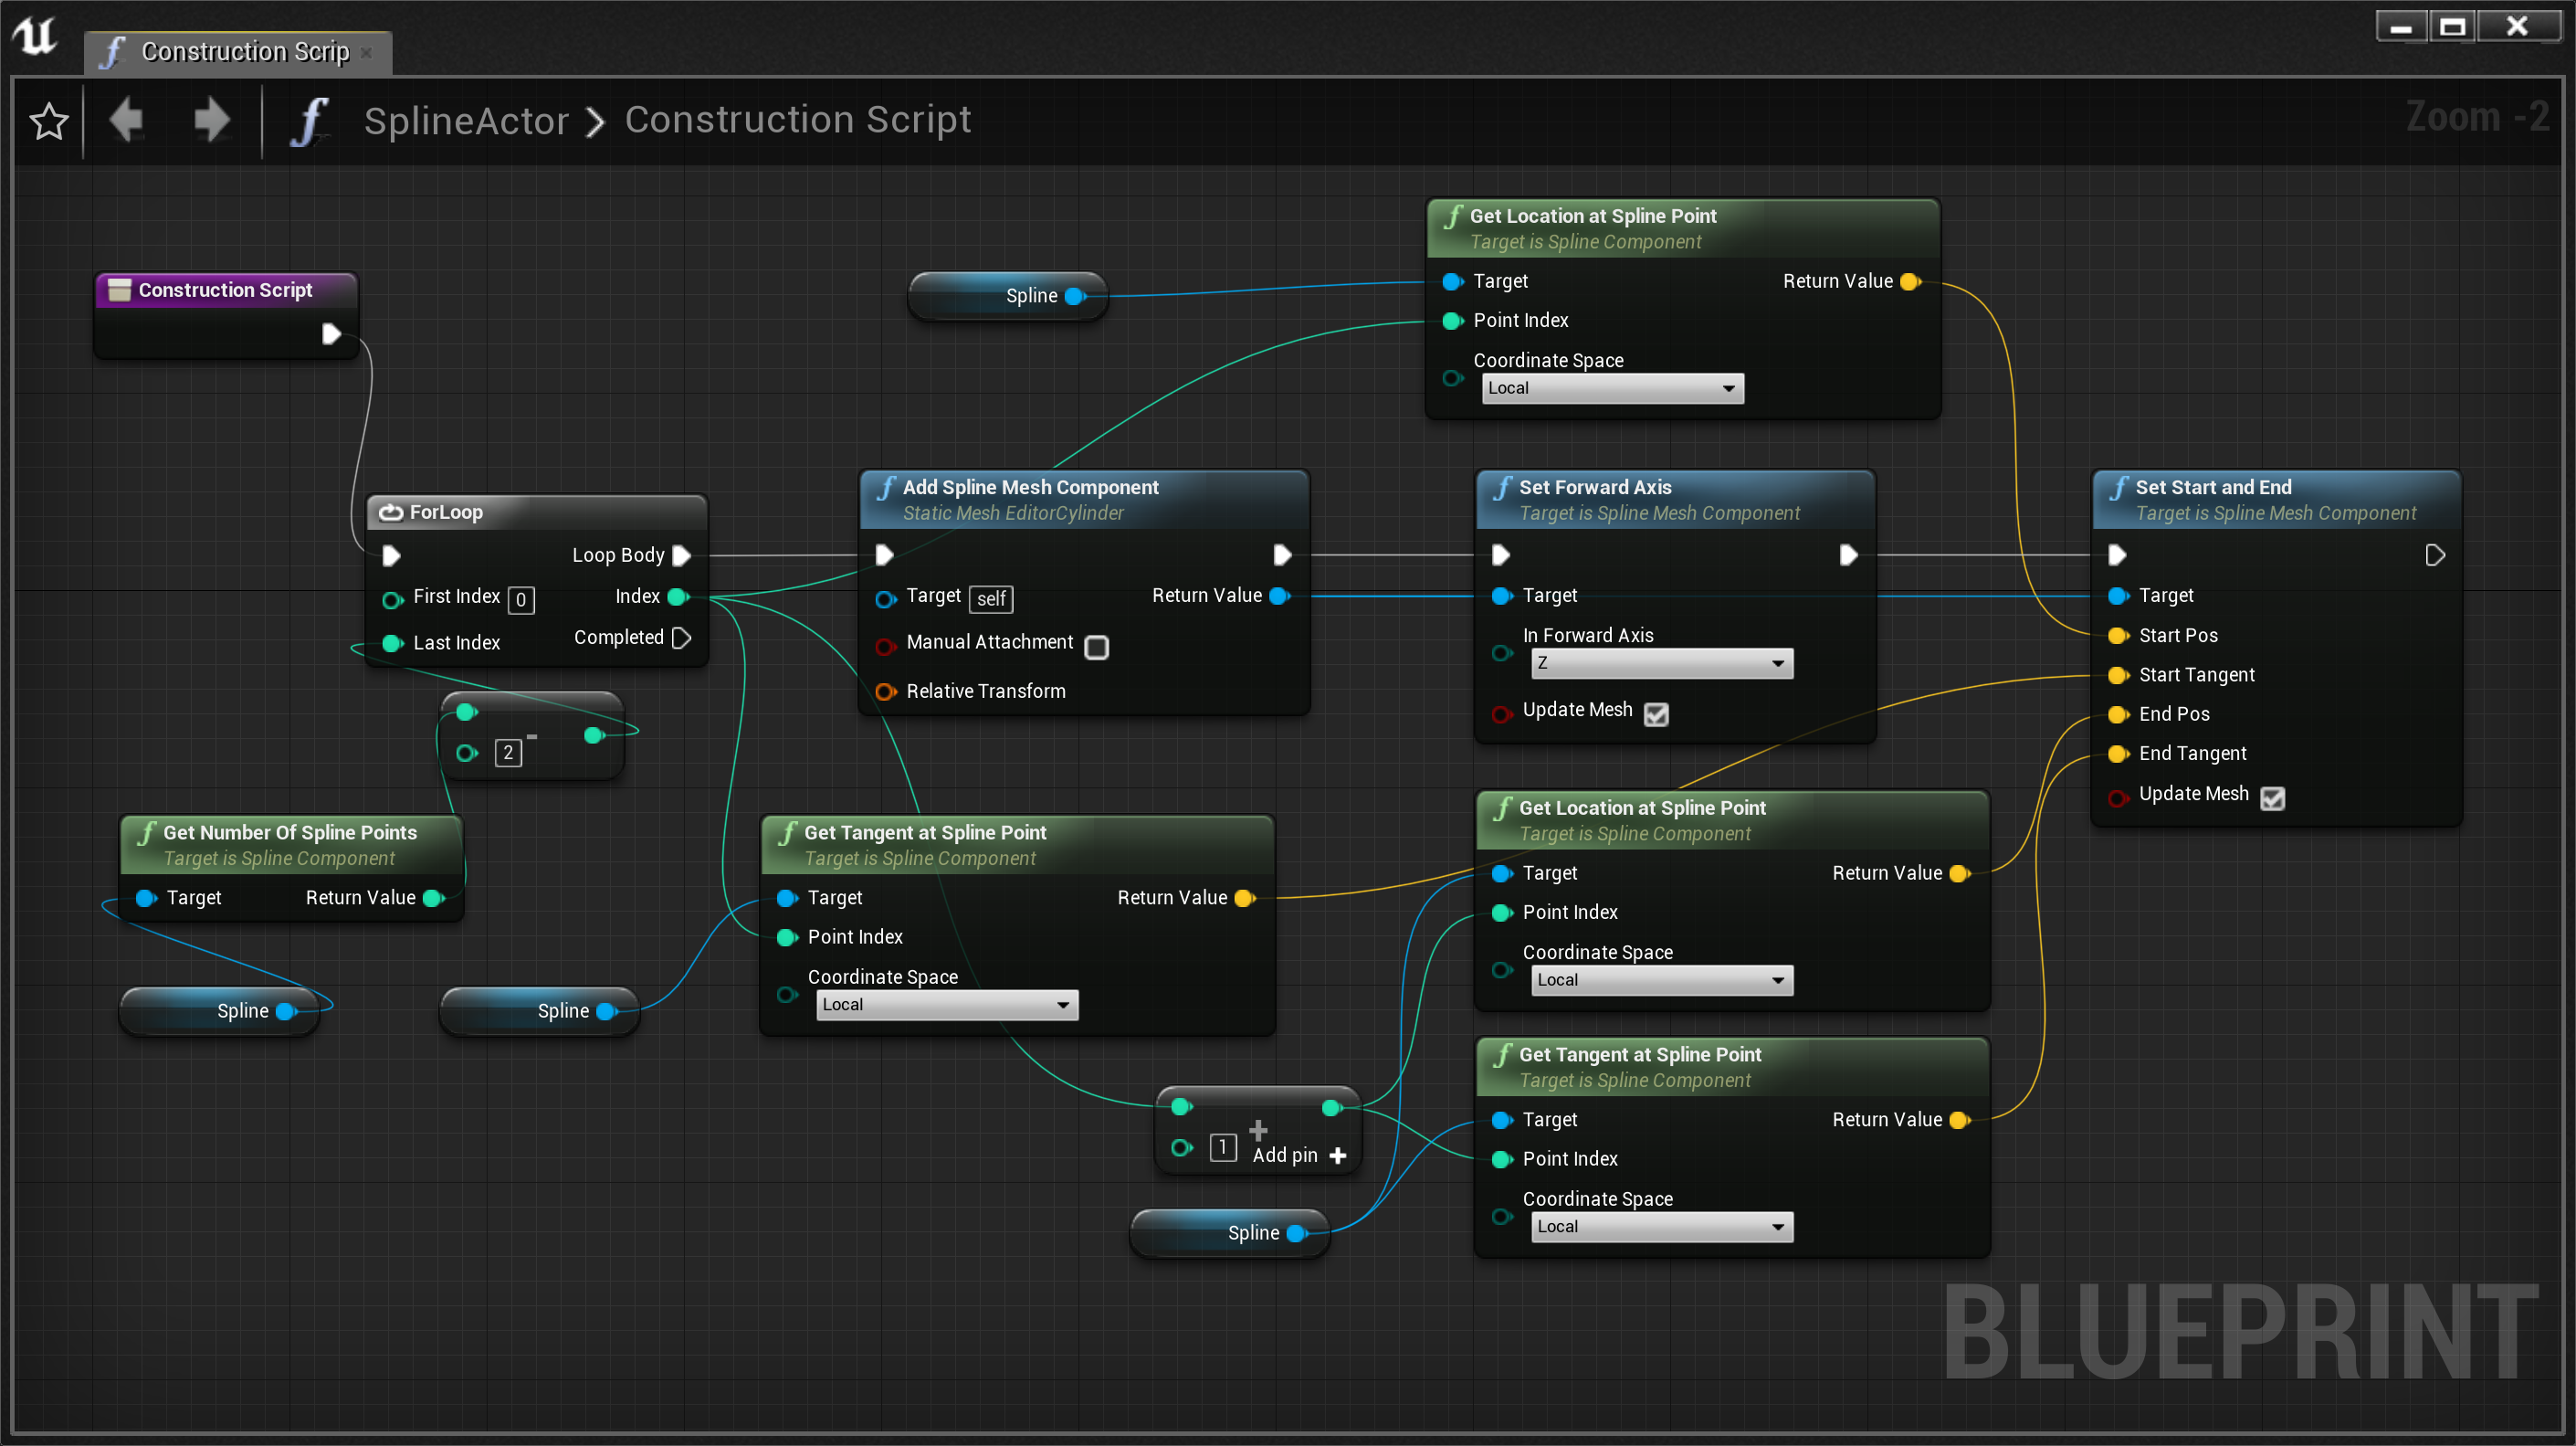
\includegraphics[width=\textwidth]{spline-component}
	\caption{Spline Actor construction script logic}
	\label{fig:spline-component}
\end{figure}
\par
Blueprint Spline Component is a component for creating paths. The path is comprised of points and a spline connecting them. This component has two primary uses \citeyeartitlexamkinline{spline-component}. Moving an actor across the spline or repeating actors across the spline. In this project the ability of the spline component to repeat actors along a path is utilized. A new Actor Blueprint is created and a Spline Component is added to the root of it. Logic is added to the construction script function to add a spline mesh of a cylinder for each spline point. The start of the cylinder spline mesh is the current spline point and the end for the spline mesh is the next spline point. The construction script function is called whever the actor is added to the scene or modified \Cref{fig:spline-component}. The end result is a Static Cable Actor that can have segments added and modified from the UE4 Editor. This actor is used for the static cabling in the scene and is replicated for every individual cable.
\subsection{Air inlet and outlet tubing}
ChemProFXi chemical detector has an air inlet port through which air to be analyzed comes in and an outlet port for the analyzed air to leave the device from. These ports need to be connected to the air outside of the vehicle. This is done by using PTFE tubing which is chemically inert and will not interact with gasses. The PTFE tubing needs to be simulated in the virtual environment. This is done with the use of the Static Cable Actor from the previous section. A different mesh in the shape of an open cylinder is used and its surface material is changed to resemble PTFE tubing. The outlet is routed to the outside of the vehicle and the inlet is left inside the vehicle for testing purposes.
\section{Creating a context for training}
The virtual scene contains the required devices and interaction capabilities. However further meaning needs to be added to the application for training purposes. This is done by creating objectives for the user to complete. The goal of the objectives is to get the user familiarised with the equipment and prepared for common scenarios encountered in real world use.
\par
Objectives need to be completed in series. The user is given visual objective instructions either with text or by highlighting scene objects of importance. Upon following the instructions the objective is complete and another one will be presented to the user. Logic for displaying instructions and logic for tracking if an objective is completed need to be tightly coupled together to ensure consistency.
\subsection{Tracking progess}
Tracking progress is the proccess of recording the state of objective completion. The application starts with a default first objective assigned. When certain interactions between objects in the scene occur the objective is changed and objectives interested in that change are notified via an event. The best place for objective tracking is in the Player State Blueprint since it is designed for holding player state and has access to all other objects in the scene.
\par
Objective tracking begins by creating a new Blueprint from the PlayerState base Blueprint. The PlayerState Blueprint is designed to store the state of each player in a multi-player or single-player environment. A new instance of this Blueprint is created for every player and only the server or the player itself can modify values of the instance. Other players are able to read values from it, but not modify them.
\begin{figure}[H]
	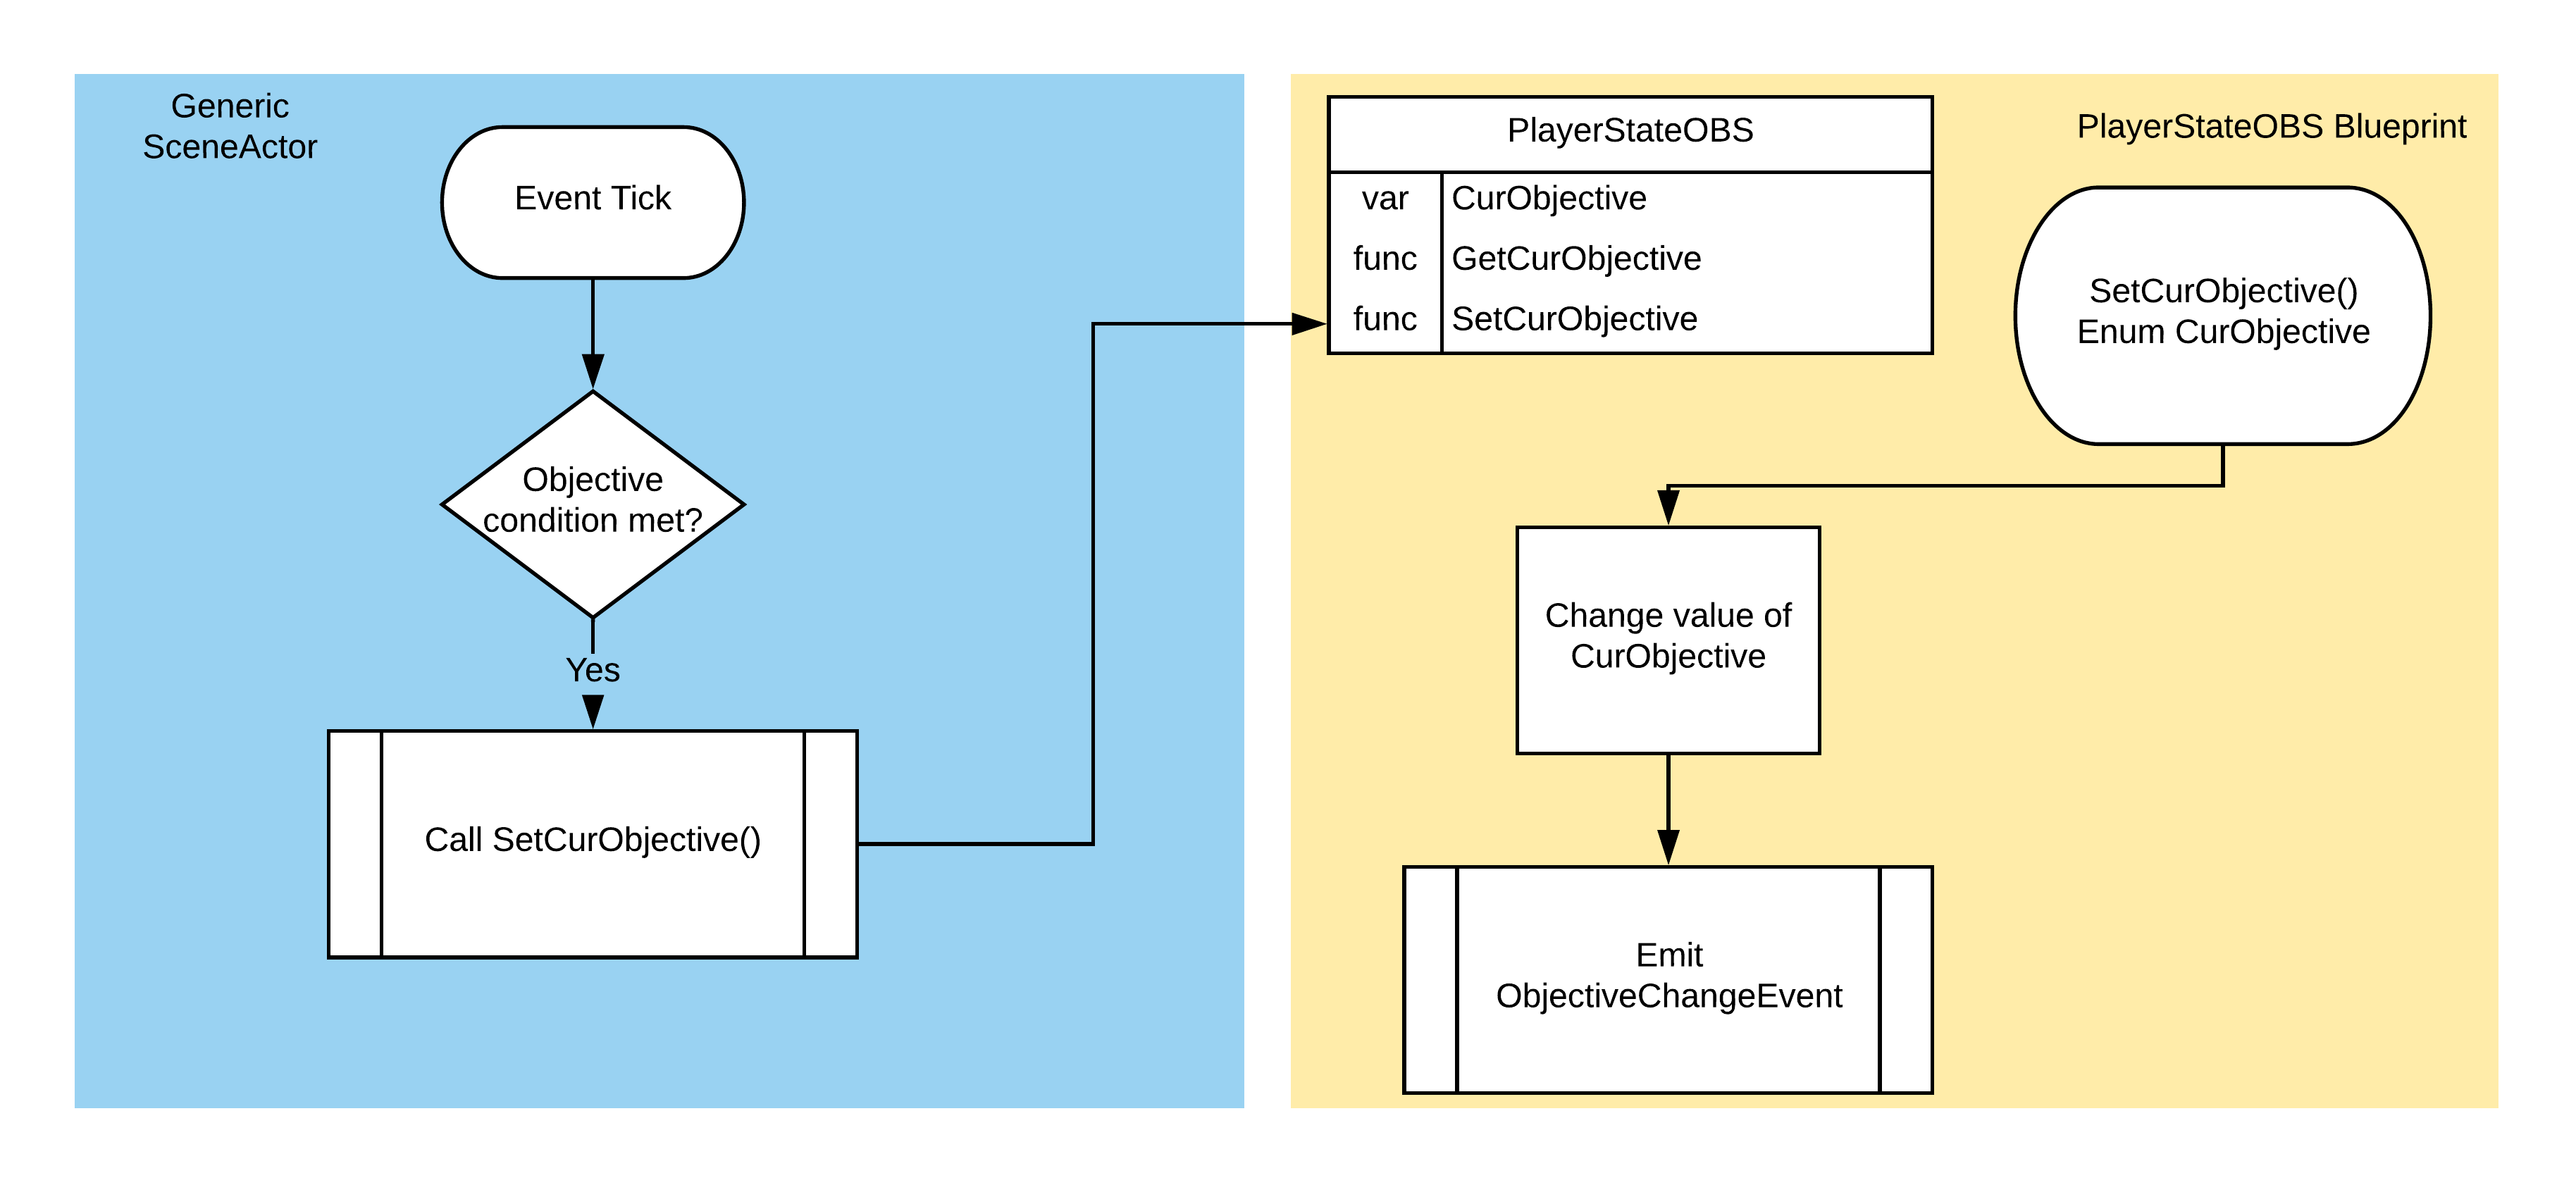
\includegraphics[width=\textwidth]{player-state}
	\caption{PlayerState Blueprint logic diagram for objective tracking}
	\label{fig:player-state}
\end{figure}
\par
To track the progress a new variable is added to the new PlayerState Blueprint that holds the current objective. The type of this variable is an Objectives Enum. This Enum type contains all the possible ojective key names. Two functions are then added to the blueprint, one for getting the current objective enum and another for changing the current objective enum value. Actors in the scene that participate in the objectives are able to get a reference of the PlayerState and call the SetCurObjective function which changes the value of the current objective. Additionally this function emits an event which is used by actors to update their own state whenever an objective changes \Cref{fig:player-state}.
\par
With the current implementation whenever the application is restarted all progress will be reset because it is kept in the memory. To be able to persist the progress tracking over application restarts the SaveGame Blueprint is used. This blueprint is used to create save slots and store variables in them. These slots persist over restarts and can be loaded with each application start. The value stored is the current objective enum, therefore the application resumes to the last objective the user was on before exiting. \citeyeartitlexamk{save-game}
\subsection{Objective instructions}
Instructions about the different objectives need to be provided to the application users. Without such instructions users can become unaware of what is required of them to do. These instructions should contain the steps required to complete the current objective. Additionally basic information about the system that is relative to the current objective can be given. This section covers the different methods used to provide instructions and information to the user.
\begin{figure}[H]
	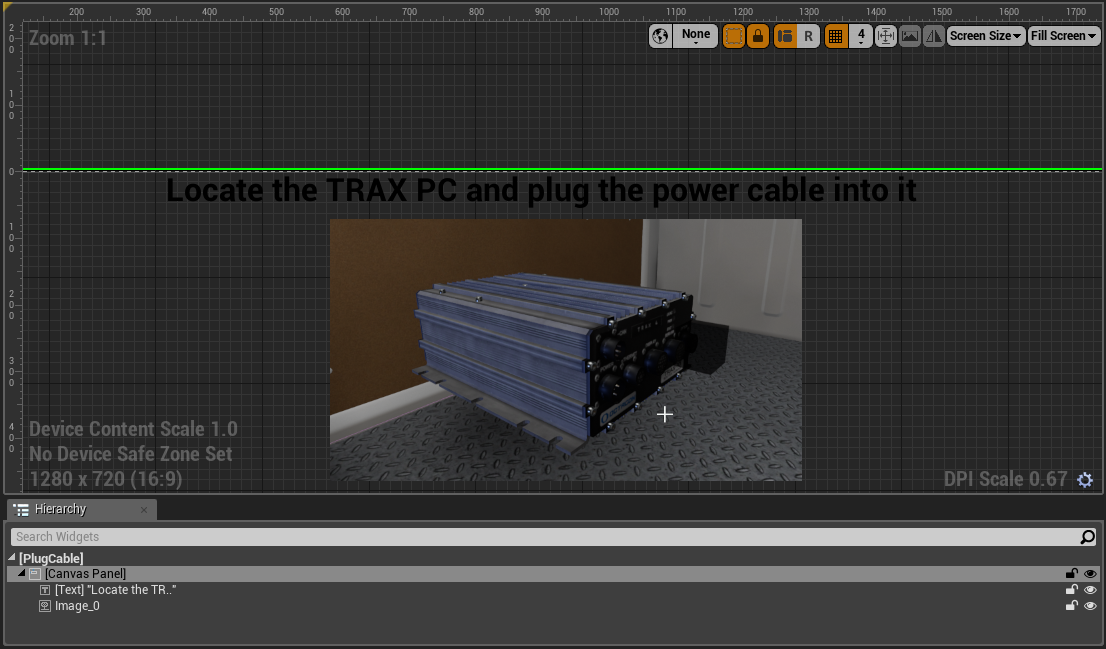
\includegraphics[width=\textwidth]{user-widget}
	\caption{UserWidget containing text and an Image element}
	\label{fig:user-widget}
\end{figure}
\par
The primary media types for instructions are text and images. These media types are two dimensional which makes Widgets a good candidate for the delivery of instructions. A virtual widescreen display will be utilised to show these instructions. Firstly a UserWidget is created for every instruction. Each UserWidget contains text and image elements that guide the user and explain what actions need to be taken. These widgets will not be modified on runtime and will not contain logic. Secondly a new WidgetComponent is created and named ScreenComponent. It contains a white Image element which is used for the text background. Furthermore all the UserWidgets created earlier are added to a WidgetSwitcher component, which itself is added to the ScreenComponent. The WidgetSwitcher component is a simple component which is used to control what is shown from the list of its children components. Lastly the ScreenWidget is listening to objective change events and commands the WidgetSwitcher which instruction widget should be shown. After performing this setup the 2D behavior of the ScreenWidget is complete.
\begin{figure}[H]
	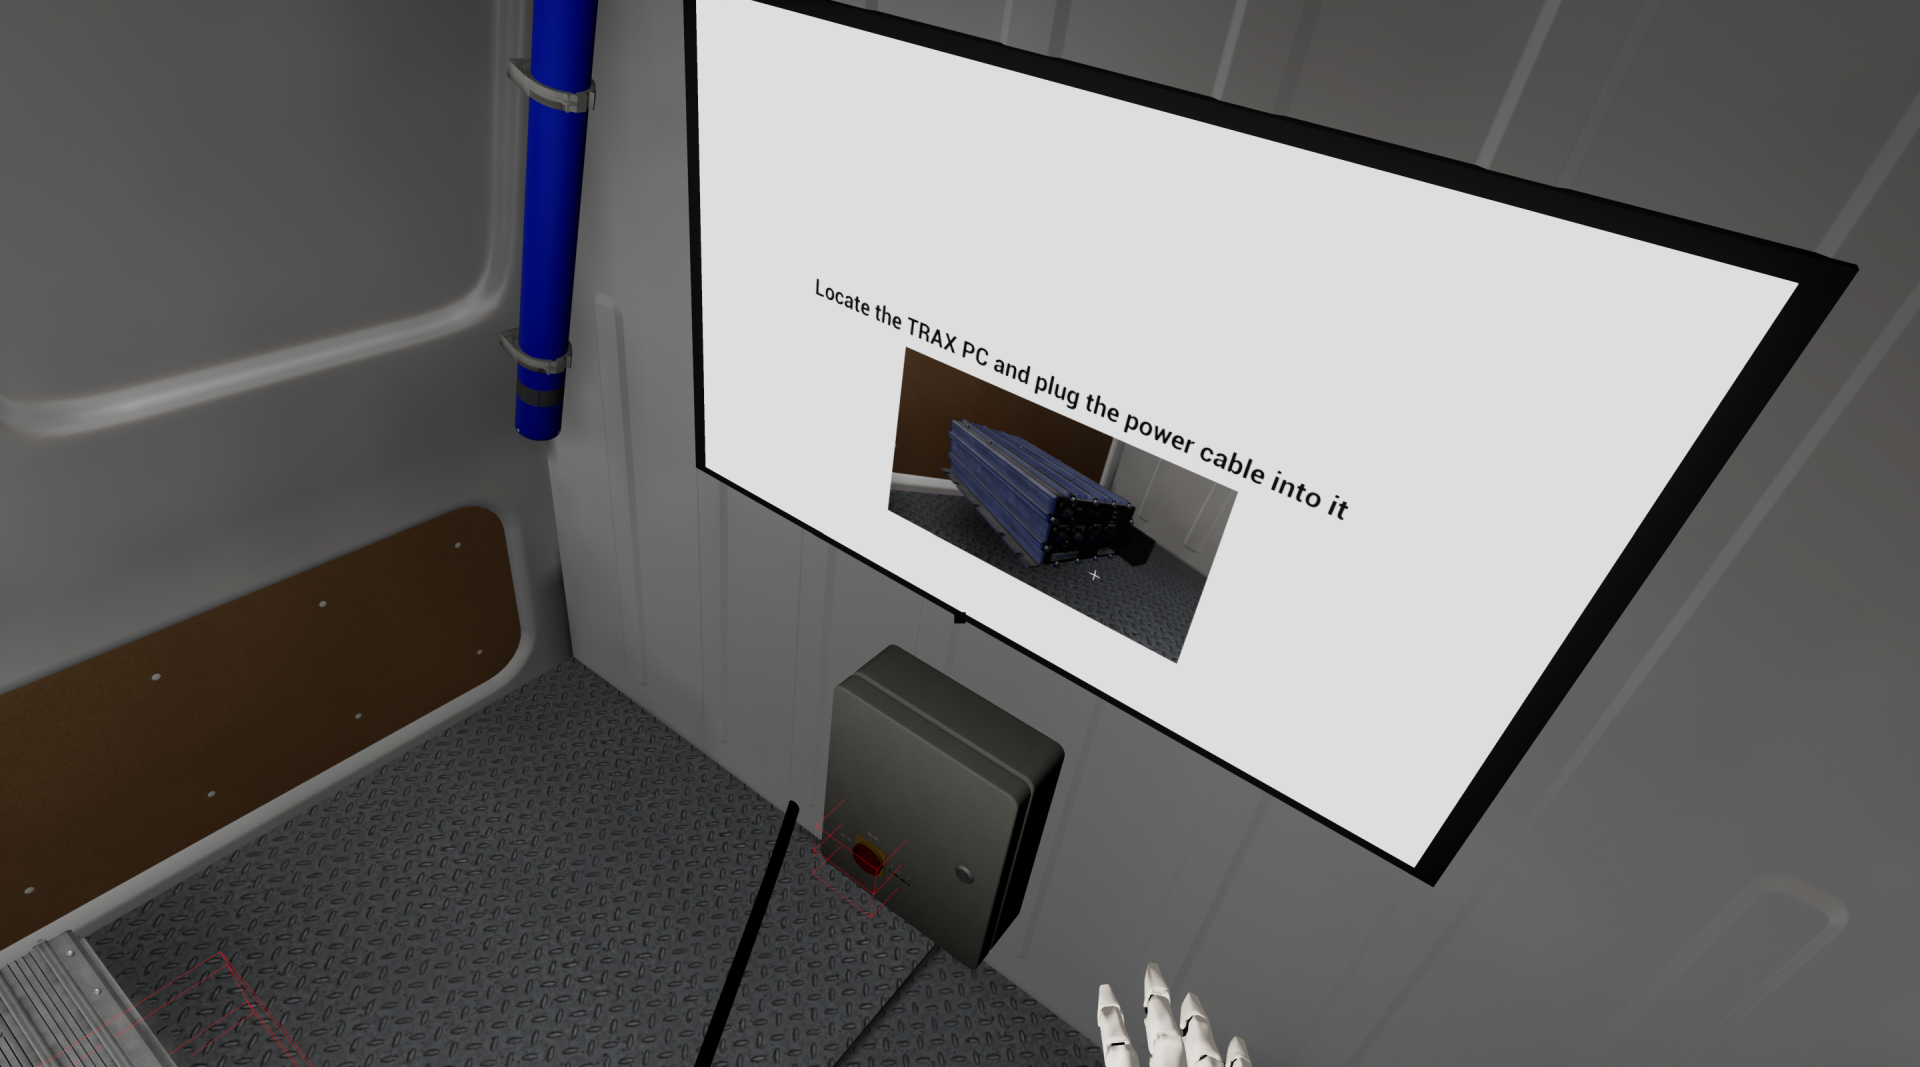
\includegraphics[width=\textwidth]{screen-component}
	\caption{ScreenComponent added to the scene}
	\label{fig:screen-component}
\end{figure}
\par
The ScreenWidget component needs to be added to the scene in order to be visible to the user. This is done by creating a new Actor Component which contains a 3D model of a touch screen and a WidgetComponent wrapping the ScreenWidget. The WidgetComponent is aligned with the surface of the 3D screen model which makes it appear as if the screen is projecting the instructions. Finally the Actor Component is added to the scene in a place where it can be seen by the user \Cref{fig:screen-component}.
\subsection{Visual and auditory cues for events}
User interaction with the virtual environment can lead to events occuring. Visual or auditory cues are needed to signal the user that such events are taking place. These cues can be considered as a feedback to the user when the environment has been changed in an impactful way. A simple example of such feedback is when a device is turned on and shortly after the device status LED starts flashing and it also starts emitting operational noise. This type of feedback is not directly related to the motor input from the user, but more so to the change of state in the environment.
\par
Events on devices can be generated either by a change of the device's own state change or by a change of the global state. An example of a device state change is when a device is turned on. An example of a global state change is when a device alarms, resulting in alarm sound and visualization coming from the toughbook laptop.
\par
Visualizing of events is accomplished by changing the visual appearance of the scene by adding, removing or modifying scene actors. One visualization tool used for real life sensor devices is LEDs that indicate status of the device. This is replicated in UE by using a PointLight as an LED light source and setting its visibility on or off depending on the virtual device status. This method is quite intuitive for the user as it is similar to real life visualization. Another visualization method used in this project is the display of text and images with Widget Components. This method was further discussed in the previous section.
\par
Sound effects can offer better immersion by simulating sounds that are present in the real ObSAS environment. Additional information can be also provided to trainees with the use of sound. Playing sounds in Unreal Engine begins by importing a Waveform Audio File(WAV) of the sound effect as an asset. This asset can be then added to the scene with the use of a Sound Cue Component. This type of component is used to modify audio playback by changing aspects such as playback speed, frequency, volume, pitch and others. The Sound Cue Component also adds spatialization to the sound source. This means that when a user is further from the sound source the sound will get quieter and vice versa when closer. Additionally there are sound volume differences between the left and right stereo channels depending on where the user is looking relative to the sound source. This makes it possible to locate the direction of the source.
\section{Building and distributing the application}

\par
\chapter{\texorpdfstring{Results and conclusion}{results-conclusion}}

\newpage

\nocite{*}
\AtBeginEnvironment{thebibliography}{\linespread{1}\selectfont}
\bibliography{references}

\end{document}
